% =====================================================================
%  Projekt inżynierski - plik główny (wersja robocza)
%  Ustawienia zgodne z wytycznymi "Jak napisać pracę inżynierską?":
%  czcionka szeryfowa 12 pt, spis treści, podpisy pod rysunkami
%  i tabelami bez kropki na końcu, Literatura bez numeru w spisie treści.
%  Strona tytułowa: wg wzoru wydziału Strona-tytulowa-I-stopien.doc.
% =====================================================================
\documentclass[12pt,a4paper,oneside]{report}

\usepackage[T1]{fontenc}
\usepackage[utf8]{inputenc}
\usepackage[polish]{babel}
% Times: newtx (Overleaf), w razie braku - mathptmx
\IfFileExists{newtxtext.sty}{\usepackage{newtxtext,newtxmath}}{\usepackage{mathptmx}}
\usepackage[a4paper,left=3cm,right=2.5cm,top=2.5cm,bottom=2.5cm]{geometry}
\usepackage{setspace}
\onehalfspacing
\usepackage{microtype}

\usepackage{graphicx}
\usepackage{booktabs}
\usepackage{tabularx}
\usepackage{multirow}
\usepackage{array}
\usepackage[table]{xcolor}
\usepackage{float}
\usepackage{tikz}
\usetikzlibrary{positioning,arrows.meta,fit,calc,shapes.geometric}
\usepackage{amsmath}
\usepackage{url}
\usepackage[hidelinks]{hyperref}

% --- Rozmieszczanie obiektów pływających: mniej stron z samymi rysunkami,
%     strony z obiektami wyrównane do góry ---
\renewcommand{\topfraction}{0.9}
\renewcommand{\bottomfraction}{0.8}
\renewcommand{\textfraction}{0.07}
\renewcommand{\floatpagefraction}{0.8}
\setcounter{topnumber}{3}
\setcounter{bottomnumber}{2}
\setcounter{totalnumber}{4}
\makeatletter
\setlength{\@fptop}{0pt}
\setlength{\@fpsep}{14pt plus 1fil}
\setlength{\@fpbot}{0pt plus 1fil}
\makeatother

% --- Podpisy: pod obiektem, "Rysunek 3.1. Opis", bez kropki na końcu ---
\usepackage[labelsep=period,font=small,labelfont=bf,justification=centering,
            skip=6pt]{caption}
\captionsetup[table]{position=bottom}
\captionsetup[lstlisting]{position=bottom}

% --- Listingi (kod) z obsługą polskich znaków ---
\usepackage{listings}
\renewcommand{\lstlistingname}{Listing}
\renewcommand{\lstlistlistingname}{Spis listingów}
\lstset{
  basicstyle=\ttfamily\footnotesize,
  columns=fullflexible, keepspaces=true,
  breaklines=true, breakatwhitespace=false,
  frame=tb, framesep=4pt, xleftmargin=0pt,
  numbers=left, numberstyle=\tiny\color{gray}, numbersep=6pt,
  showstringspaces=false, tabsize=2,
  commentstyle=\color{black!60}\itshape,
  keywordstyle=\bfseries,
  literate={ą}{{\k{a}}}1 {ć}{{\'c}}1 {ę}{{\k{e}}}1 {ł}{{\l{}}}1 {ń}{{\'n}}1
           {ó}{{\'o}}1 {ś}{{\'s}}1 {ź}{{\'z}}1 {ż}{{\.z}}1
           {Ą}{{\k{A}}}1 {Ć}{{\'C}}1 {Ę}{{\k{E}}}1 {Ł}{{\L{}}}1 {Ń}{{\'N}}1
           {Ó}{{\'O}}1 {Ś}{{\'S}}1 {Ź}{{\'Z}}1 {Ż}{{\.Z}}1
           {‖}{{$\|$}}1 {→}{{$\rightarrow$}}1
}

% --- Pomocnicze makra ---
\newcommand{\kod}[1]{\texttt{#1}}          % nazwy plików, poleceń, funkcji
\newcommand{\ang}[1]{\textit{#1}}          % termin angielski (kursywa)
\newcommand{\douzup}[1]{\colorbox{yellow!40}{\small [do uzupełnienia: #1]}}
\newcolumntype{L}{>{\raggedright\arraybackslash}X}

% --- Dane strony tytułowej (UZUPEŁNIĆ pola oznaczone \douzup) ---
\newcommand{\tytulPL}{Analiza podatności protokołów sieciowych i~błędów logicznych w~implementacjach kryptograficznych}
\newcommand{\tytulEN}{Vulnerability analysis of network protocols and logic flaws in cryptographic implementations}
\newcommand{\autorpracy}{Daniel Kubiela}
\newcommand{\wydzial}{Wydział Informatyki, Elektroniki i~Telekomunikacji}
\newcommand{\instytut}{\douzup{nazwa instytutu}}
\newcommand{\kierunek}{\douzup{nazwa kierunku}}
\newcommand{\opiekun}{\douzup{stopień lub tytuł, imię i nazwisko}}
\newcommand{\rokpracy}{\douzup{rok}}
\newcommand{\tytulowa}{\fontfamily{phv}\selectfont}  % krój strony tytułowej (Helvetica)

\addto\captionspolish{\renewcommand{\bibname}{Literatura}}

\begin{document}

% ---------------- Strona tytułowa ----------------
% Odwzorowanie wzoru wydziału "Strona-tytulowa-I-stopien.doc"
% (https://iet.agh.edu.pl/egzamin-dyplomowy/). Położenie elementów i wielkości
% pisma zmierzone ze wzoru; logo wyciągnięte z pliku wzoru. Krój wzoru (Inter)
% zastąpiono Helvetiką (helvet), dostępną w każdej dystrybucji TeX.
% Pola do uzupełnienia są zdefiniowane w preambule (\instytut, \kierunek, \opiekun, \rokpracy).
\begin{titlepage}
\begin{tikzpicture}[remember picture, overlay,
    tp/.style={inner sep=0pt, outer sep=0pt, font=\tytulowa}]
  % logo z napisem "Akademia Górniczo-Hutnicza im. Stanisława Staszica w Krakowie"
  \node[tp, anchor=north] at ($(current page.north)+(0,-97.5pt)$)
    {
\includegraphics[width=399.9pt]{rysunki/agh-logo.jpg}};
  % wydział
  \node[tp, anchor=base] at ($(current page.north)+(0,-308.4pt)$)
    {\fontsize{11}{13.3}\selectfont\bfseries\MakeUppercase{\wydzial}};
  % instytut
  \node[tp, anchor=base] at ($(current page.north)+(0,-333.7pt)$)
    {\fontsize{11}{13.3}\selectfont INSTYTUT \instytut};
  % rodzaj pracy
  \node[tp, anchor=base] at ($(current page.north)+(0,-386.3pt)$)
    {\fontsize{18}{21.7}\selectfont Projekt dyplomowy};
  % tytuł w języku oryginalnym (polskim) i w języku angielskim
  \node[tp, anchor=north, text width=453pt, align=center] at ($(current page.north)+(0,-424.5pt)$)
    {\fontsize{16}{19.3}\selectfont\strut\tytulPL\par\strut\tytulEN\par};
  % autor, kierunek, opiekun
  \node[tp, anchor=base west] at ($(current page.north west)+(71pt,-603.7pt)$)
    {\fontsize{11}{13.3}\selectfont Autor:};
  \node[tp, anchor=base west] at ($(current page.north west)+(212.7pt,-603.7pt)$)
    {\fontsize{11}{13.3}\selectfont \autorpracy};
  \node[tp, anchor=base west] at ($(current page.north west)+(71pt,-617.0pt)$)
    {\fontsize{11}{13.3}\selectfont Kierunek studiów:};
  \node[tp, anchor=base west] at ($(current page.north west)+(212.7pt,-617.0pt)$)
    {\fontsize{11}{13.3}\selectfont \kierunek};
  \node[tp, anchor=base west] at ($(current page.north west)+(71pt,-630.3pt)$)
    {\fontsize{11}{13.3}\selectfont Opiekun pracy:};
  \node[tp, anchor=base west] at ($(current page.north west)+(212.7pt,-630.3pt)$)
    {\fontsize{11}{13.3}\selectfont \opiekun};
  % miejsce i rok
  \node[tp, anchor=base] at ($(current page.north)+(0,-670.2pt)$)
    {\fontsize{11}{13.3}\selectfont Kraków, \rokpracy};
\end{tikzpicture}
\end{titlepage}

\tableofcontents

% Rozdział 1 - do napisania po ukończeniu części praktycznej
\chapter{Wstęp}\label{ch:wstep}
\section{Uzasadnienie wyboru tematu}
\section{Cel i zakres pracy}
\section{Pytania badawcze}
\section{Struktura pracy}

% Rozdział 2 - do napisania po ukończeniu części praktycznej
\chapter{Model zagrożeń i podstawy kryptograficzne}\label{ch:podstawy}
\section{Etapy ataku w ujęciu modelu Cyber Kill Chain}\label{sec:killchain}
\section{Poufność, integralność i autentyczność danych}\label{sec:cia}
\section{Tryby pracy szyfrów: strumieniowe, CBC, AEAD}\label{sec:tryby}
\section{Funkcje skrótu i kody uwierzytelniające}\label{sec:skroty}
\section{Funkcje wyprowadzania klucza: compute-hard i memory-hard}\label{sec:kdf}
\section{Mechanizmy negocjacji parametrów sesji w protokole TLS}\label{sec:tls}

% =====================================================================
%  Rozdział 3 - Środowisko badawcze (wersja robocza)
% =====================================================================
\chapter{Środowisko badawcze}\label{ch:srodowisko}

Rozdział opisuje stanowisko, na którym przeprowadzono wszystkie badania praktyczne: wymagania postawione środowisku, topologię sieci laboratoryjnej, konfigurację maszyn i~usług, platformę sprzętową wykorzystaną w~pomiarach wydajnościowych oraz przyjętą metodykę pomiarów. Opisana konfiguracja jest wspólna dla rozdziałów \ref{ch:ataki}--\ref{ch:obrona}; w~kolejnych rozdziałach przywoływane są jedynie elementy istotne dla danego eksperymentu.

% ---------------------------------------------------------------------
\section{Założenia i wymagania}\label{sec:wymagania}

Środowisko zaprojektowano tak, aby umożliwiało bezpieczne odtwarzanie badanych scenariuszy, rejestrację całego ruchu sieciowego oraz porównywanie mechanizmów w~wariancie podatnym i~poprawionym. Ze względu na dostępne zasoby całość musiała zmieścić się na jednym komputerze, który pełni jednocześnie funkcję stanowiska do pomiarów wydajności kryptoanalizy z~wykorzystaniem procesora graficznego (ang. \ang{Graphics Processing Unit}, GPU). Sformułowane wymagania oraz sposób ich realizacji zestawiono w~tabeli~\ref{tab:wymagania}.

\begin{table}[htbp]
\centering\small
\begin{tabularx}{\textwidth}{@{}>{\raggedright\arraybackslash}p{4.2cm}L@{}}
\toprule
\textbf{Wymaganie} & \textbf{Sposób realizacji} \\
\midrule
Izolacja ruchu badawczego & ruch badawczy przesyłany wyłącznie w~wydzielonej sieci wewnętrznej hipernadzorcy, bez routingu do sieci zewnętrznej \\
Rozdzielenie ról & osobne maszyny wirtualne dla klienta, serwera usług, czujnika systemu detekcji włamań i~napastnika \\
Warianty porównawcze & każdy badany mechanizm uruchomiony równolegle w~wersji podatnej i~poprawionej na tym samym serwerze \\
Obserwowalność & czujnik z~interfejsem w~trybie nasłuchu (ang. \ang{promiscuous mode}) i~zapisem ruchu do plików \kod{pcap} \\
Powtarzalność & migawki stanu maszyn, automatyzacja pomiarów skryptami, stałe ziarna generatorów losowych, wielokrotne powtarzanie pomiarów \\
Niezależność pomiarów wydajności & pomiary GPU wykonywane bezpośrednio w~systemie hosta przy wyłączonych maszynach wirtualnych \\
Ograniczone zasoby & klony połączone maszyn wirtualnych zamiast pełnych kopii dysków \\
\bottomrule
\end{tabularx}
\caption{Wymagania stawiane środowisku badawczemu i~sposób ich realizacji}
\label{tab:wymagania}
\end{table}

% ---------------------------------------------------------------------
\section{Topologia stanowiska laboratoryjnego}\label{sec:topologia}

Laboratorium sieciowe zbudowano w~hipernadzorcy Oracle VirtualBox w~wersji 7.2.8~\cite{virtualbox}, uruchomionym na komputerze z~systemem Windows~11~Pro. Topologię stanowiska przedstawiono na rysunku~\ref{rys:topologia}. Składa się ono z~czterech maszyn wirtualnych połączonych wewnętrzną siecią VirtualBox o~nazwie \kod{labnet} (adresacja 10.10.10.0/24). Sieć ta nie posiada bramy ani połączenia z~siecią zewnętrzną -- cały ruch generowany w~trakcie badań pozostaje w~jej obrębie.

\begin{figure}[htbp]
\centering
\resizebox{\textwidth}{!}{%
\begin{tikzpicture}[
  font=\footnotesize,
  vm/.style={draw, rounded corners=3pt, minimum width=3.3cm, minimum height=1.55cm,
             align=center, fill=white},
  szyna/.style={line width=1pt},
  >={Stealth[length=2mm]}]
  % maszyny wirtualne
  \node[vm] (kali)   at (0,0)    {\textbf{Napastnik} (\kod{kali})\\10.10.10.10\\Kali Linux 2026.2};
  \node[vm] (client) at (3.8,0)  {\textbf{Klient} (\kod{client})\\10.10.10.20\\skrypty pomiarowe};
  \node[vm] (server) at (7.6,0)  {\textbf{Serwer} (\kod{server})\\10.10.10.30\\Docker: aplikacja, 2$\times$TLS};
  \node[vm, line width=1.2pt] (sensor) at (11.4,0) {\textbf{Czujnik} (\kod{sensor})\\10.10.10.40\\Snort 3, tcpdump};
  \node[font=\scriptsize] at (11.4,1.08) {tryb nasłuchu};
  % szyny
  \draw[szyna] (-1.65,-1.45) -- (13.05,-1.45);
  \draw[szyna, dashed] (-1.65,-2.2) -- (13.05,-2.2);
  \foreach \m in {kali,client,server,sensor}{
    \draw ($(\m.south)+(-0.35,0)$) -- ($(\m.south)+(-0.35,-0.675)$) node[circle,fill,inner sep=1.3pt]{};
    \draw[dashed] ($(\m.south)+(0.35,0)$) -- ($(\m.south)+(0.35,-1.425)$) node[circle,fill,inner sep=1.3pt]{};
  }
  % legenda
  \draw[szyna] (-1.6,-2.65) -- (-0.9,-2.65) node[right,font=\scriptsize]{sieć wewnętrzna \kod{labnet} 10.10.10.0/24 (karta \kod{enp0s3}) -- ruch badawczy};
  \draw[szyna,dashed] (-1.6,-3.05) -- (-0.9,-3.05) node[right,font=\scriptsize]{NAT VirtualBox (karta \kod{enp0s8}) -- instalacja pakietów i~zarządzanie};
  % host
  \node[draw, rounded corners=3pt, minimum width=14.7cm, minimum height=0.9cm, align=center,
        fill=black!4] (host) at (5.7,-4.0)
    {\textbf{Host}: Windows 11 Pro, VirtualBox 7.2.8 \quad$\cdot$\quad stanowisko GPU: Hashcat 7.1.2, NVIDIA GeForce GTX 1660};
  \draw[dashed,<->] (12.3,-2.2) -- (12.3,-3.55) node[midway,left,font=\scriptsize,align=right]{SSH z~hosta:\\127.0.0.1:2220/2230/2240};
\end{tikzpicture}}
\caption{Topologia stanowiska laboratoryjnego}
\label{rys:topologia}
\end{figure}

Każda maszyna posiada dwie karty sieciowe. Pierwsza, \kod{enp0s3}, jest podłączona do sieci \kod{labnet} i~ma statycznie przypisany adres; to przez nią przechodzi cały ruch badawczy. Druga, \kod{enp0s8}, korzysta z~translacji adresów (NAT) VirtualBox i~służy wyłącznie do instalacji pakietów oraz zarządzania maszynami przez protokół SSH. Dostęp z~hosta realizowany jest przez przekierowanie portów 127.0.0.1:2220, 2230 i~2240 odpowiednio do maszyn klienta, serwera i~czujnika. Na karcie \kod{labnet} czujnika włączono tryb nasłuchu zarówno w~ustawieniach VirtualBox (zezwolenie na cały ruch), jak i~w~systemie operacyjnym, dzięki czemu czujnik rejestruje ruch wymieniany między pozostałymi maszynami, mimo że sam nie jest jego stroną. Parametry maszyn zestawiono w~tabeli~\ref{tab:maszyny}.

\begin{table}[htbp]
\centering\small
\begin{tabularx}{\textwidth}{@{}l l l c L@{}}
\toprule
\textbf{Maszyna} & \textbf{Adres} & \textbf{System} & \textbf{RAM / vCPU} & \textbf{Rola w~badaniach} \\
\midrule
\kod{kali}   & 10.10.10.10 & Kali Linux 2026.2      & 3~GB / 2 & stacja napastnika \\
\kod{client} & 10.10.10.20 & Ubuntu Server 24.04.5  & 1~GB / 1 & klient usług, uruchamianie skryptów pomiarowych \\
\kod{server} & 10.10.10.30 & Ubuntu Server 24.04.5  & 2~GB / 2 & usługi w~wariancie podatnym i~poprawionym \\
\kod{sensor} & 10.10.10.40 & Ubuntu Server 24.04.5  & 2~GB / 2 & czujnik systemu detekcji włamań, rejestracja ruchu \\
\bottomrule
\end{tabularx}
\caption{Maszyny wirtualne stanowiska laboratoryjnego}
\label{tab:maszyny}
\end{table}

Maszyny klienta, serwera i~czujnika utworzono jako klony połączone (ang. \ang{linked clones}) jednej maszyny bazowej \kod{ubuntu-base} z~systemem Ubuntu Server 24.04~\cite{ubuntuserver}. Klon połączony przechowuje jedynie różnice względem dysku maszyny bazowej, dlatego bezpośrednio po utworzeniu zajmuje kilkadziesiąt megabajtów zamiast kilku gigabajtów. Punktem wyjścia dla klonów jest migawka \kod{czysta-baza} maszyny bazowej. Po zainstalowaniu oprogramowania każdej z~maszyn wykonano migawkę \kod{baseline}, do której można wrócić przed powtórzeniem eksperymentu. Budowę stanowiska zautomatyzowano: skrypt PowerShell uruchamiany na hoście tworzy klony i~konfiguruje karty sieciowe, a~skrypty uruchamiane w~maszynach nadają nazwy hostów, adresy w~sieci \kod{labnet} oraz instalują oprogramowanie właściwe dla roli maszyny.

% ---------------------------------------------------------------------
\section{Konfiguracja maszyn i usług}\label{sec:konfiguracja}

\subsection{Serwer usług}\label{sec:serwer}

Wszystkie badane usługi uruchomiono na maszynie \kod{server} jako kontenery zarządzane narzędziem Docker Compose~\cite{docker}. Takie rozwiązanie pozwala uruchomić na jednym serwerze usługi o~skrajnie różnych wymaganiach -- w~tym serwer zbudowany na przestarzałej bibliotece kryptograficznej -- bez wzajemnego wpływu na konfigurację systemu. Definicję usług przedstawiono na listingu~\ref{lst:compose}, a~ich przeznaczenie w~tabeli~\ref{tab:uslugi}.

\begin{lstlisting}[float=htbp,language={},caption={Definicja usług serwera laboratoryjnego (plik \kod{docker-compose.yml}, fragment)},label={lst:compose}]
services:
  webapp:                       # aplikacja testowa (HTTP)
    build: ./webapp
    ports: ["5000:5000"]
  modern-tls:                   # serwer TLS - konfiguracja utwardzona
    image: nginx:1.27-alpine
    volumes:
      - ./nginx-modern/nginx.conf:/etc/nginx/nginx.conf:ro
      - ./certs:/certs:ro
    ports: ["443:443"]
  legacy-tls:                   # serwer TLS - konfiguracja przestarzała
    build: ./legacy-tls         # OpenSSL 1.0.2u kompilowany ze źródeł
    volumes: ["./certs:/certs:ro"]
    ports: ["4433:4433"]
\end{lstlisting}

\begin{table}[htbp]
\centering\small
\begin{tabularx}{\textwidth}{@{}l l L@{}}
\toprule
\textbf{Port} & \textbf{Usługa} & \textbf{Przeznaczenie} \\
\midrule
5000/tcp & aplikacja testowa (Flask) & ciasteczka sesyjne i~podpisy żądań w~wariancie podatnym i~poprawionym (rozdz.~\ref{ch:ataki}) \\
443/tcp  & nginx 1.27 & serwer TLS w~konfiguracji utwardzonej: tylko TLS~1.2 i~1.3 oraz zestawy szyfrów z~uwierzytelnieniem \\
4433/tcp & OpenSSL 1.0.2u (\kod{s\_server}) & serwer TLS w~konfiguracji przestarzałej: protokoły od SSLv3 do TLS~1.2, w~tym zestawy z~trybem CBC i~szyfrem RC4 \\
\bottomrule
\end{tabularx}
\caption{Usługi uruchomione na serwerze laboratoryjnym}
\label{tab:uslugi}
\end{table}

Aplikację testową napisano w~języku Python z~użyciem szkieletu Flask~\cite{flask} i~biblioteki kryptograficznej PyCryptodome~\cite{pycryptodome}. Aplikacja udostępnia trzy pary mechanizmów, w~których wariant podatny i~poprawiony różnią się wyłącznie zastosowaną konstrukcją kryptograficzną (tabela~\ref{tab:aplikacja}). Klucze szyfrujące (128-bitowe, osobne dla każdego wariantu) oraz sekret używany do podpisywania żądań generowane są losowo przy każdym uruchomieniu aplikacji. Aplikację udostępniono celowo bez warstwy TLS, aby jej ruch był w~całości widoczny dla czujnika. Treść ciasteczka sesyjnego ma postać \kod{user=<nazwa>;admin=0;uid=1001}; pole \kod{admin} decyduje o~dostępie do funkcji administracyjnych, co pozwala ocenić nie tylko to, czy modyfikacja została przyjęta, ale też jaki ma skutek.

\begin{table}[htbp]
\centering\small
\begin{tabularx}{\textwidth}{@{}>{\raggedright\arraybackslash}p{2.9cm}LLc@{}}
\toprule
\textbf{Mechanizm} & \textbf{Wariant podatny} & \textbf{Wariant poprawiony} & \textbf{Podrozdz.} \\
\midrule
ciasteczko sesyjne (szyfr strumieniowy) & AES-128-CTR bez kodu uwierzytelniającego; \kod{/ctr/login}, \kod{/ctr/profile} & AES-128-GCM; \kod{/secure/login}, \kod{/secure/profile} & \ref{sec:ctr} \\
ciasteczko sesyjne (szyfr blokowy) & AES-128-CBC bez kodu uwierzytelniającego; \kod{/login}, \kod{/profile} & AES-128-GCM (jw.) & \ref{sec:cbc} \\
podpis żądania API & SHA-256(sekret~$\|$~wiadomość); \kod{/api/sample}, \kod{/api/transfer} & HMAC-SHA-256; \kod{/api/secure/sample}, \kod{/api/secure/transfer} & \ref{sec:lenext} \\
\bottomrule
\end{tabularx}
\caption{Pary mechanizmów aplikacji testowej}
\label{tab:aplikacja}
\end{table}

Do badania negocjacji parametrów sesji przygotowano dwa serwery TLS posługujące się tym samym, samopodpisanym certyfikatem (klucz RSA 2048~bitów, nazwa \kod{lab-server}). Serwer w~konfiguracji utwardzonej to nginx~\cite{nginxssl}, w~którym dopuszczono wyłącznie protokoły TLS~1.2 i~1.3 oraz zestawy szyfrów z~uwierzytelnieniem (listing~\ref{lst:nginx}). Serwer w~konfiguracji przestarzałej to program \kod{s\_server} z~biblioteki OpenSSL~\cite{openssl} w~wersji 1.0.2u, skompilowanej ze źródeł w~obrazie kontenera i~uruchomionej z~możliwie szeroką listą zestawów szyfrów (listing~\ref{lst:legacy}).

\begin{lstlisting}[float=htbp,language={},caption={Konfiguracja protokołów i~szyfrów serwera utwardzonego (\kod{nginx.conf}, fragment)},label={lst:nginx}]
listen 443 ssl;
ssl_certificate     /certs/server.crt;
ssl_certificate_key /certs/server.key;
ssl_protocols TLSv1.2 TLSv1.3;
ssl_ciphers ECDHE-ECDSA-AES128-GCM-SHA256:ECDHE-RSA-AES128-GCM-SHA256:
            ECDHE-RSA-AES256-GCM-SHA384:ECDHE-RSA-CHACHA20-POLY1305;
ssl_prefer_server_ciphers on;
\end{lstlisting}

\begin{lstlisting}[float=htbp,language={},caption={Uruchomienie serwera w~konfiguracji przestarzałej (\kod{entrypoint.sh})},label={lst:legacy}]
exec /opt/openssl-legacy/bin/openssl s_server \
  -accept 4433 \
  -cert /certs/server.crt -key /certs/server.key \
  -cipher 'ALL:RC4:!aNULL:!eNULL' \
  -www
\end{lstlisting}

\subsection{Maszyna klienta}\label{sec:klient}

Maszyna \kod{client} służy jako klient wszystkich badanych usług i~miejsce uruchamiania skryptów pomiarowych. Oprócz systemowej biblioteki OpenSSL w~wersji 3.0.13 zainstalowano na niej równolegle, w~katalogu \kod{/opt/openssl-legacy}, bibliotekę OpenSSL 1.0.2u. Instalacja równoległa była konieczna, ponieważ współczesne wersje biblioteki nie pozwalają już nawiązać połączenia z~użyciem protokołów SSLv3, TLS~1.0 i~TLS~1.1, co uniemożliwiłoby zbadanie, które z~tych wersji akceptuje serwer. Skrypty pomiarowe uruchamiane na kliencie napisano w~języku Python (wersja 3.12.3) z~wykorzystaniem wyłącznie biblioteki standardowej oraz w~języku powłoki Bash.

\subsection{Czujnik systemu detekcji włamań}\label{sec:czujnik}

Na maszynie \kod{sensor} zainstalowano system detekcji włamań (ang. \ang{Intrusion Detection System}, IDS) Snort w~wersji 3.12.2.0~\cite{snort3}, skompilowany ze źródeł. Na czas kompilacji przydział pamięci maszyny zwiększono do 4~GB. Konfiguracja czujnika składa się z~pliku bazowego \kod{snort.lua}, pliku z~ustawieniami laboratorium \kod{lab.lua} (wczytywanego opcją \kod{--tweaks lab}) oraz pliku reguł własnych \kod{local.rules}. W~pliku \kod{lab.lua} włączono inspektor \kod{arp\_spoof} i~wpisano do niego poprawne powiązania adresów IP z~adresami sprzętowymi kart sieciowych klienta i~serwera, odczytane z~tablicy sąsiadów czujnika. Szczegóły konfiguracji detekcji opisano w~podrozdziale~\ref{sec:ids}. Do zapisu ruchu w~plikach \kod{pcap} wykorzystywano program tcpdump~\cite{tcpdump}. Zapisane pliki analizowano następnie offline, co pozwala wielokrotnie uruchamiać detekcję na identycznym materiale.

\subsection{Maszyna napastnika}\label{sec:napastnik}

Maszyna \kod{kali} z~dystrybucją Kali Linux 2026.2~\cite{kali} pełni w~topologii rolę stacji napastnika podłączonej do tego samego segmentu sieci co ofiara. W~eksperymentach opisanych w~kolejnych rozdziałach ruch testowy generowano jednak z~maszyny klienta, co upraszczało automatyzację pomiarów i~nie wpływało na ich wynik: z~punktu widzenia serwera i~czujnika istotna jest treść przesyłanych komunikatów, a~nie maszyna, z~której pochodzą.

\subsection{Wersje oprogramowania}

Wersje oprogramowania wszystkich maszyn zestawiono w~tabeli~\ref{tab:wersje}. Wykaz sporządzono po zakończeniu instalacji i~nie zmieniano go w~trakcie badań.

\begin{table}[htbp]
\centering\small
\begin{tabularx}{\textwidth}{@{}l L l@{}}
\toprule
\textbf{Maszyna} & \textbf{Oprogramowanie} & \textbf{Wersja} \\
\midrule
\kod{server}, \kod{client}, \kod{sensor} & Ubuntu Server / jądro Linux & 24.04.5 LTS / 6.8.0-147 \\
\kod{server} & Docker / Docker Compose & 29.1.3 / 2.40.3 \\
\kod{server} & nginx (obraz kontenera) & 1.27 \\
\kod{server}, \kod{client} & OpenSSL (instalacja przestarzała) & 1.0.2u \\
\kod{client} & OpenSSL (systemowy) / Python & 3.0.13 / 3.12.3 \\
\kod{sensor} & Snort & 3.12.2.0 \\
\kod{kali} & Kali Linux / jądro Linux & 2026.2 / 6.19.14 \\
host & Windows / VirtualBox & 11 Pro / 7.2.8 \\
\bottomrule
\end{tabularx}
\caption{Wersje oprogramowania stanowiska laboratoryjnego}
\label{tab:wersje}
\end{table}

\subsection{Problemy napotkane podczas budowy stanowiska}

Budowa stanowiska wymagała rozwiązania kilku problemów wynikających głównie z~ograniczeń sprzętowych i~domyślnych ustawień narzędzi. Zestawiono je w~tabeli~\ref{tab:problemy}, ponieważ mają znaczenie dla powtórzenia konfiguracji na innym komputerze.

\begin{table}[htbp]
\centering\small
\begin{tabularx}{\textwidth}{@{}>{\raggedright\arraybackslash}p{4.1cm}>{\raggedright\arraybackslash}p{4.6cm}L@{}}
\toprule
\textbf{Problem} & \textbf{Przyczyna} & \textbf{Rozwiązanie} \\
\midrule
instalator systemu nie uruchamiał się z~obrazu ISO & przestarzała wersja VirtualBox (6.1) & aktualizacja do wersji 7.2 \\
błąd \kod{VERR\_DISK\_FULL} przy uruchamianiu klonów & brak miejsca na dysku systemowym, pełne kopie dysków & klony połączone i~przeniesienie maszyn na osobny dysk \\
brak serwera SSH w~maszynie bazowej & instalacja nienadzorowana bez pakietu OpenSSH & doinstalowanie \kod{openssh-server} przed klonowaniem \\
klony bez łączności sieciowej & konfiguracja sieci powiązana z~adresem MAC maszyny bazowej & konfiguracja sieci według nazw interfejsów (\kod{enp0s3}, \kod{enp0s8}) \\
brak klienta SSH w~systemie hosta & nieudana instalacja funkcji opcjonalnej systemu Windows & instalacja pakietu Win32-OpenSSH \\
\bottomrule
\end{tabularx}
\caption{Problemy napotkane podczas budowy stanowiska i~ich rozwiązania}
\label{tab:problemy}
\end{table}

% ---------------------------------------------------------------------
\section{Platforma sprzętowa do badań wydajnościowych}\label{sec:platforma}

Badania wydajności kryptoanalizy offline (rozdział~\ref{ch:gpu}) przeprowadzono na tym samym komputerze, na którym działa laboratorium sieciowe, ale bezpośrednio w~systemie hosta, a~nie w~maszynach wirtualnych. Parametry platformy zestawiono w~tabeli~\ref{tab:platforma}.

\begin{table}[htbp]
\centering\small
\begin{tabularx}{\textwidth}{@{}>{\raggedright\arraybackslash}p{4.3cm}L@{}}
\toprule
\textbf{Element} & \textbf{Parametry} \\
\midrule
Procesor (CPU) & AMD Ryzen 5 5600, 6 rdzeni, 12 wątków \\
Pamięć operacyjna & 16~GB \\
Karta graficzna (GPU) & NVIDIA GeForce GTX 1660, 6~GB pamięci GDDR5 \\
System operacyjny & Windows 11 Pro \\
Sterownik karty graficznej & NVIDIA 610.88 (CUDA 13.3) \\
Narzędzie do kryptoanalizy & Hashcat 7.1.2 \\
Obliczenia na CPU & Intel CPU Runtime for OpenCL \\
Pliki testowe & VeraCrypt 1.26.29, KeePassXC 2.8.0, 7-Zip \\
Generowanie skrótów Argon2 & Python 3.12, biblioteka \kod{argon2-cffi} \\
\bottomrule
\end{tabularx}
\caption{Platforma sprzętowa i~programowa badań wydajnościowych}
\label{tab:platforma}
\end{table}

Do pomiarów wykorzystano narzędzie Hashcat~\cite{hashcat}, które pozwala uruchomić te same algorytmy zarówno na karcie graficznej, jak i~na procesorze. Obliczenia na karcie graficznej wykonywane były przez interfejs CUDA, a~na procesorze -- przez interfejs OpenCL, udostępniony przez środowisko Intel CPU Runtime for OpenCL. Pliki testowe, czyli kontenery szyfrowane, bazy haseł i~zaszyfrowane archiwa, utworzono w~programach VeraCrypt~\cite{veracrypt}, KeePassXC~\cite{keepassxc} oraz 7-Zip, a~dane potrzebne do ataku offline wyodrębniono z~nich pomocniczymi narzędziami \kod{7z2hashcat} i~\kod{keepass2john}.

Na czas pomiarów wydajności wszystkie maszyny wirtualne były wyłączone, aby nie konkurowały z~badanymi obliczeniami o~zasoby procesora i~pamięci. W~trakcie pomiarów na karcie graficznej co 2~sekundy zapisywano jej temperaturę, taktowanie, pobór mocy i~obciążenie (program \kod{nvidia-smi}). Pozwoliło to wykluczyć wpływ dławienia termicznego na wyniki.

% ---------------------------------------------------------------------
\section{Metodyka pomiarów}\label{sec:metodyka}

Wszystkie eksperymenty przeprowadzono według wspólnego schematu, przedstawionego na rysunku~\ref{rys:przebieg}. Każdy pomiar poprzedzało przygotowanie środowiska: uruchomienie potrzebnych maszyn i~usług, a~w~przypadku badań ruchu sieciowego -- rozpoczęcie jego zapisu na czujniku. Sam pomiar wykonywał skrypt, który zapisywał zarówno wynik zbiorczy, jak i~surowe dane każdej próby. Wyniki weryfikowano, a~następnie archiwizowano i~opracowywano w~postaci tabel i~wykresów.

\begin{figure}[htbp]
\centering
\begin{tikzpicture}[
  font=\footnotesize,
  krok/.style={draw, rounded corners=3pt, minimum width=2.5cm, minimum height=1.0cm,
               align=center, fill=black!4},
  opis/.style={align=center, text width=2.6cm, font=\scriptsize},
  >={Stealth[length=2mm]}]
  \node[krok] (k1) at (0,0)     {\textbf{Przygotowanie}};
  \node[krok] (k2) at (3.05,0)  {\textbf{Pomiar}};
  \node[krok] (k3) at (6.1,0)   {\textbf{Rejestracja}};
  \node[krok] (k4) at (9.15,0)  {\textbf{Weryfikacja}};
  \node[krok] (k5) at (12.2,0)  {\textbf{Opracowanie}};
  \foreach \a/\b in {k1/k2,k2/k3,k3/k4,k4/k5} \draw[->] (\a) -- (\b);
  \node[opis, below=2mm of k1] {migawka \kod{baseline}, uruchomienie usług, zapis ruchu na czujniku};
  \node[opis, below=2mm of k2] {skrypt pomiarowy, stałe ziarno, seria prób};
  \node[opis, below=2mm of k3] {pliki CSV i~TXT, pliki \kod{pcap}, log karty graficznej};
  \node[opis, below=2mm of k4] {powtórzenia, porównanie z~wartością oczekiwaną};
  \node[opis, below=2mm of k5] {archiwum wyników, tabele i~wykresy};
\end{tikzpicture}
\caption{Schemat przebiegu pojedynczego eksperymentu}
\label{rys:przebieg}
\end{figure}

Przyjęto następujące zasady szczegółowe:
\begin{itemize}
  \item \textbf{Porównanie wariantów.} Każdy mechanizm badano w~wariancie podatnym i~poprawionym w~identycznych warunkach, tym samym skryptem. Dzięki temu różnica w~wynikach wynika wyłącznie z~zastosowanej konstrukcji kryptograficznej lub konfiguracji.
  \item \textbf{Automatyzacja.} Pomiary wykonywały skrypty zestawione w~tabeli~\ref{tab:skrypty}. Skrypty zapisywały surowe dane każdej próby, co umożliwiało późniejsze sprawdzenie wyniku zbiorczego.
  \item \textbf{Powtarzalność.} Serie losowych prób wykonywano ze stałym ziarnem generatora pseudolosowego (20261025 dla rozdziału~\ref{ch:ataki}, 20261029 dla zbioru testowego w~rozdziale~\ref{ch:obrona}), dzięki czemu można je dokładnie powtórzyć. Pomiary wydajności powtarzano trzykrotnie (dla funkcji Argon2 -- dwukrotnie) i~podawano wartość średnią.
  \item \textbf{Weryfikacja narzędzi.} Przed uruchomieniem na stanowisku każdy skrypt sprawdzano na lokalnej kopii aplikacji testowej. Tam, gdzie było to możliwe, wynik pomiaru porównywano z~wartością wynikającą z~budowy badanego mechanizmu.
  \item \textbf{Analiza offline.} Ruch sieciowy zapisywano do plików \kod{pcap}, a~detekcję uruchamiano na zapisanym ruchu. Pozwala to porównywać różne wersje reguł na identycznym materiale wejściowym.
  \item \textbf{Archiwizacja.} Wszystkie wyniki (pliki CSV i~TXT, pliki \kod{pcap}, logi) archiwizowano w~repozytorium Git projektu wraz ze skryptami, które je wytworzyły.
\end{itemize}

\begin{table}[htbp]
\centering\small
\begin{tabularx}{\textwidth}{@{}>{\raggedright\arraybackslash}p{5.2cm}l L c@{}}
\toprule
\textbf{Skrypt} & \textbf{Maszyna} & \textbf{Przeznaczenie} & \textbf{Rozdz.} \\
\midrule
\kod{r4-skan-tls.sh}, \kod{r4-scsv.sh} & klient & wersje protokołu akceptowane przez serwery TLS, reakcja na sygnał obniżenia wersji & \ref{ch:ataki} \\
\kod{r4-pomiar-integralnosci.py} & klient & odporność ciasteczek i~podpisów na modyfikację & \ref{ch:ataki} \\
\kod{pomiar-bench.ps1} & host & test wydajności GPU z~zapisem parametrów karty & \ref{ch:gpu} \\
\kod{pomiar-veracrypt.ps1}, \kod{pomiar-hash.ps1} & host & prędkość ataku na własne pliki testowe & \ref{ch:gpu} \\
\kod{pomiar-gpu-cpu.ps1} & host & porównanie GPU i~CPU dla wybranych algorytmów & \ref{ch:gpu} \\
\kod{gen-argon2.py}, \kod{pomiar-argon2.ps1} & host & skalowanie funkcji Argon2 względem pamięci & \ref{ch:gpu} \\
\kod{local.rules}, \kod{lab.lua} & czujnik & reguły i~konfiguracja detekcji & \ref{ch:obrona} \\
\kod{r6-gen-zbior.py}, \kod{r6-entropia.py}, \kod{r6-realne.py} & host & zbiór testowy i~klasyfikacja plików zaszyfrowanych & \ref{ch:obrona} \\
\bottomrule
\end{tabularx}
\caption{Skrypty i~pliki konfiguracyjne wykorzystane w~pomiarach}
\label{tab:skrypty}
\end{table}

% =====================================================================
%  Rozdział 4 - wersja robocza do przeredagowania
%  Dane: wyniki/R4 (pomiary 25.10.2026, test uzupełniający SCSV 8.11.2026)
%  Skróty TLS, CTR, CBC, GCM, HMAC, AEAD rozwinąć przy pierwszym użyciu
%  w rozdziale 2 - tu rozwinięte są tylko te, które mogą tam nie wystąpić.
% =====================================================================
\chapter{Analiza ataków na mechanizmy negocjacji sesji i~integralność danych}\label{ch:ataki}

W rozdziale przedstawiono wyniki eksperymentów dotyczących dwóch grup zagrożeń: ingerencji w~negocjację parametrów sesji TLS oraz modyfikacji danych chronionych kryptograficznie bez kontroli integralności. Wszystkie eksperymenty przeprowadzono na stanowisku opisanym w~rozdziale~\ref{ch:srodowisko}, według schematu z~podrozdziału~\ref{sec:metodyka}. Każdy mechanizm badano w~wariancie podatnym i~poprawionym, tym samym skryptem i~w~tych samych warunkach. Przegląd eksperymentów zawiera tabela~\ref{tab:r4-przeglad}. Właściwości mechanizmów, z~których wynikają obserwowane zachowania, omówiono w~rozdziale~\ref{ch:podstawy}; w~tym rozdziale opisano sposób pomiaru i~uzyskane wyniki.

\begin{table}[htbp]
\centering\small
\begin{tabularx}{\textwidth}{@{}c >{\raggedright\arraybackslash}p{3.3cm} L >{\raggedright\arraybackslash}p{2.3cm} >{\raggedright\arraybackslash}p{2.6cm}@{}}
\toprule
\textbf{Podrozdz.} & \textbf{Badany mechanizm} & \textbf{Wariant podatny / poprawiony} & \textbf{Liczba prób} & \textbf{Miara} \\
\midrule
\ref{sec:arp}    & podszycie w~protokole ARP & -- / detekcja inspektorem \kod{arp\_spoof} & 3 ramki & liczba alarmów \\
\ref{sec:tlsneg} & negocjacja wersji TLS & OpenSSL 1.0.2u / nginx 1.27 & 10 + 4 połączenia & wersja, zestaw szyfrów, reakcja na SCSV \\
\ref{sec:ctr}    & ciasteczko sesyjne, szyfr strumieniowy & AES-128-CTR / AES-128-GCM & $2\times200$ + 2 & odsetek przyjętych modyfikacji \\
\ref{sec:cbc}    & ciasteczko sesyjne, szyfr blokowy & AES-128-CBC / AES-128-GCM & $2\times200$ + 1 & odsetek przyjętych modyfikacji \\
\ref{sec:lenext} & podpis żądania API & SHA-256(sekret~$\|$~wiadomość) / HMAC-SHA-256 & $2\times5$ & reakcja serwera \\
\bottomrule
\end{tabularx}
\caption{Przegląd eksperymentów rozdziału~\ref{ch:ataki}}
\label{tab:r4-przeglad}
\end{table}

% ---------------------------------------------------------------------
\section{Wykrywalność podszycia w~protokole ARP}\label{sec:arp}

Ataki analizowane w~dalszej części rozdziału zakładają, że napastnik może obserwować i~modyfikować ruch między klientem a~serwerem, czyli zajmuje pozycję pośrednika (ang. \ang{man-in-the-middle}). W~sieci lokalnej pozycję tę uzyskuje się najczęściej przez wprowadzenie fałszywych powiązań do pamięci podręcznej protokołu odwzorowania adresów (ang. \ang{Address Resolution Protocol}, ARP), który nie uwierzytelnia odpowiedzi (podrozdział~\ref{sec:killchain}). Celem eksperymentu nie było przechwycenie ruchu, lecz sprawdzenie, czy taka próba jest widoczna dla czujnika systemu detekcji włamań.

\subsection*{Przebieg pomiaru}

Czujnik zapisywał ruch w~sieci \kod{labnet} programem tcpdump. Z~maszyny klienta wysłano w~odstępach około 1~s trzy ramki odpowiedzi ARP, w~których adres IP serwera (10.10.10.30) powiązano z~adresem sprzętowym (ang. \ang{Media Access Control}, MAC) karty sieciowej klienta. Powiązanie to jest sprzeczne ze wzorcem wpisanym do konfiguracji inspektora \kod{arp\_spoof} systemu Snort (tabela~\ref{tab:arp-wzorzec}). Zapisany ruch przeanalizowano następnie offline, uruchamiając Snort z~konfiguracją laboratorium.

\begin{table}[htbp]
\centering\small
\begin{tabular}{@{}lll@{}}
\toprule
\textbf{Maszyna} & \textbf{Adres IP} & \textbf{Adres MAC (wzorzec)} \\
\midrule
\kod{client} & 10.10.10.20 & \kod{08:00:27:3b:7f:6d} \\
\kod{server} & 10.10.10.30 & \kod{08:00:27:f7:36:74} \\
\bottomrule
\end{tabular}
\caption{Wzorcowe powiązania adresów wpisane do konfiguracji inspektora \kod{arp\_spoof}}
\label{tab:arp-wzorzec}
\end{table}

\subsection*{Wyniki}

Zapis ruchu z~czasu eksperymentu zawiera sześć ramek ARP (tabela~\ref{tab:arp-ramki}). Pierwsze trzy to ogłoszenia (ang. \ang{gratuitous ARP}), w~których klient rozgłasza poprawne powiązanie własnego adresu. Kolejne trzy to badane odpowiedzi, przypisujące adres serwera adresowi sprzętowemu klienta. Zestawienie ramek odczytano bezpośrednio z~pliku \kod{arp41.pcap}, a~alarmy z~wyjścia programu Snort (rysunek~\ref{rys:snort-arp}).

\begin{table}[htbp]
\centering\small
\begin{tabularx}{\textwidth}{@{}c r l l l L@{}}
\toprule
\textbf{Nr} & \textbf{Czas [s]} & \textbf{Operacja} & \textbf{Nadawca: IP} & \textbf{Nadawca: MAC} & \textbf{Alarmy} \\
\midrule
1 & 0,000 & zapytanie (ogłoszenie) & 10.10.10.20 & \kod{08:00:27:3b:7f:6d} & brak \\
2 & 0,100 & zapytanie (ogłoszenie) & 10.10.10.20 & \kod{08:00:27:3b:7f:6d} & brak \\
3 & 0,400 & zapytanie (ogłoszenie) & 10.10.10.20 & \kod{08:00:27:3b:7f:6d} & brak \\
4 & 0,825 & odpowiedź & \textbf{10.10.10.30} & \kod{08:00:27:3b:7f:6d} & 112:3, 112:4 \\
5 & 1,827 & odpowiedź & \textbf{10.10.10.30} & \kod{08:00:27:3b:7f:6d} & 112:3, 112:4 \\
6 & 2,828 & odpowiedź & \textbf{10.10.10.30} & \kod{08:00:27:3b:7f:6d} & 112:3, 112:4 \\
\bottomrule
\end{tabularx}
\caption{Ramki ARP zarejestrowane przez czujnik w~czasie eksperymentu (czas liczony od pierwszej ramki)}
\label{tab:arp-ramki}
\end{table}

\begin{figure}[htbp]
\centering
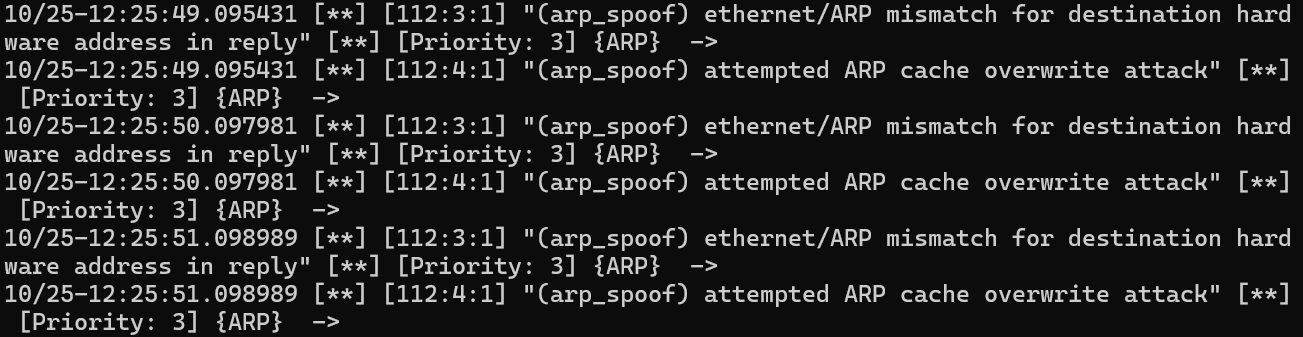
\includegraphics[width=\textwidth]{rysunki/r4-snort-arp.png}
\caption{Alarmy inspektora \kod{arp\_spoof} dla trzech odpowiedzi ARP sprzecznych ze wzorcem}
\label{rys:snort-arp}
\end{figure}

Każda z~trzech odpowiedzi wywołała dwa alarmy o~priorytecie~3, opatrzone tym samym znacznikiem czasu co ramka (łącznie sześć alarmów). Ogłoszenia klienta dotyczące jego własnego, poprawnego powiązania nie wywołały żadnego alarmu. Znaczenie obu typów alarmów podano w~tabeli~\ref{tab:arp-alarmy}.

\begin{table}[htbp]
\centering\small
\begin{tabularx}{\textwidth}{@{}l >{\raggedright\arraybackslash}p{5.1cm} L c@{}}
\toprule
\textbf{Identyfikator} & \textbf{Komunikat} & \textbf{Przyczyna w~badanej ramce} & \textbf{Liczba} \\
\midrule
112:3 & \ang{ethernet/ARP mismatch for destination hardware address in reply} & adres docelowy w~nagłówku Ethernet (rozgłoszeniowy) różni się od adresu docelowego w~treści odpowiedzi ARP & 3 \\
112:4 & \ang{attempted ARP cache overwrite attack} & odpowiedź wiąże adres IP serwera z~innym adresem MAC niż wzorcowy & 3 \\
\bottomrule
\end{tabularx}
\caption{Alarmy zgłoszone przez inspektor \kod{arp\_spoof}}
\label{tab:arp-alarmy}
\end{table}

Wynik potwierdza, że próba podszycia się pod serwer w~warstwie łącza danych pozostawia ślad wykrywalny dla czujnika: wykryto 3 z~3~badanych ramek. Skuteczność ta ma jednak dwa warunki. Po pierwsze, alarm 112:4, który bezpośrednio wskazuje na próbę nadpisania powiązania, może powstać wyłącznie dla adresów wpisanych do wzorca -- inspektor nie chroni maszyn, których powiązań nie skonfigurowano. Po drugie, alarmy w~formacie \kod{alert\_fast} nie zawierają adresów, więc ustalenie, którego powiązania dotyczyła próba, wymaga sięgnięcia do zapisu ruchu. Zachowanie inspektora wobec zwykłego ruchu sieciowego, w~tym liczbę fałszywych alarmów, oceniono w~podrozdziale~\ref{sec:ids}.

% ---------------------------------------------------------------------
\section{Negocjacja wersji protokołu TLS i~sygnalizacja obniżenia wersji}\label{sec:tlsneg}

Pośrednik w~komunikacji może próbować skłonić strony do zestawienia sesji w~najsłabszej wspólnie obsługiwanej wersji protokołu (ang. \ang{downgrade}). O~tym, czy taka próba może się powieść, decyduje przede wszystkim zbiór wersji akceptowanych przez serwer. Badanie obejmowało dwa serwery opisane w~podrozdziale~\ref{sec:serwer}: serwer w~konfiguracji przestarzałej (OpenSSL 1.0.2u, port 4433) i~serwer w~konfiguracji utwardzonej (nginx 1.27, port 443).

\subsection*{Przebieg pomiaru}

Skrypt \kod{r4-skan-tls.sh} uruchomiony na maszynie klienta próbował zestawić z~każdym serwerem połączenie w~każdej z~wersji od SSLv3 do TLS~1.3, za każdym razem dopuszczając tylko jedną wersję. Do wersji TLS~1.2 i~1.3 użyto systemowej biblioteki OpenSSL 3.0.13, a~do wersji starszych -- biblioteki OpenSSL 1.0.2u, ponieważ biblioteka współczesna nie pozwala ich już użyć. Połączenie uznawano za zaakceptowane, jeżeli strony wynegocjowały zestaw szyfrów; w~przeciwnym razie -- za odrzucone. Łącznie wykonano 10~prób połączenia.

\subsection*{Wyniki}

Wyniki zestawiono w~tabeli~\ref{tab:tls-wersje}, a~wyjście skryptu przedstawiono na rysunku~\ref{rys:skan-tls}. Serwer przestarzały zaakceptował cztery z~pięciu wersji, w~tym SSLv3. Dla wersji SSLv3, TLS~1.0 i~TLS~1.1 wynegocjował zestaw \kod{ECDHE-RSA-AES256-SHA}, czyli szyfr w~trybie CBC z~kodem uwierzytelniającym HMAC-SHA1, ponieważ zestawy z~uwierzytelnionym szyfrowaniem (ang. \ang{Authenticated Encryption with Associated Data}, AEAD) są dostępne dopiero od TLS~1.2. Odrzucenie wersji TLS~1.3 nie jest wynikiem utwardzenia, lecz braku jej implementacji w~bibliotece OpenSSL 1.0.2u. Serwer utwardzony zaakceptował wyłącznie TLS~1.2 i~1.3, w~obu przypadkach z~zestawem AEAD, co odpowiada zaleceniu wycofania wersji TLS~1.0 i~1.1 zawartemu w~RFC~8996~\cite{rfc8996}.

\begin{table}[htbp]
\centering\small
\begin{tabularx}{\textwidth}{@{}l L L@{}}
\toprule
\textbf{Wersja} & \textbf{Serwer utwardzony (nginx, :443)} & \textbf{Serwer przestarzały (OpenSSL 1.0.2u, :4433)} \\
\midrule
SSLv3   & odrzucona & zaakceptowana, \kod{ECDHE-RSA-AES256-SHA} \\
TLS~1.0 & odrzucona & zaakceptowana, \kod{ECDHE-RSA-AES256-SHA} \\
TLS~1.1 & odrzucona & zaakceptowana, \kod{ECDHE-RSA-AES256-SHA} \\
TLS~1.2 & zaakceptowana, \kod{ECDHE-RSA-AES128-GCM-SHA256} & zaakceptowana, \kod{ECDHE-RSA-AES256-GCM-SHA384} \\
TLS~1.3 & zaakceptowana, \kod{TLS\_AES\_256\_GCM\_SHA384} & odrzucona \\
\midrule
\textbf{Razem} & \textbf{2 z~5} & \textbf{4 z~5} \\
\bottomrule
\end{tabularx}
\caption{Wersje protokołu akceptowane przez serwery i~wynegocjowane zestawy szyfrów}
\label{tab:tls-wersje}
\end{table}

\begin{figure}[htbp]
\centering
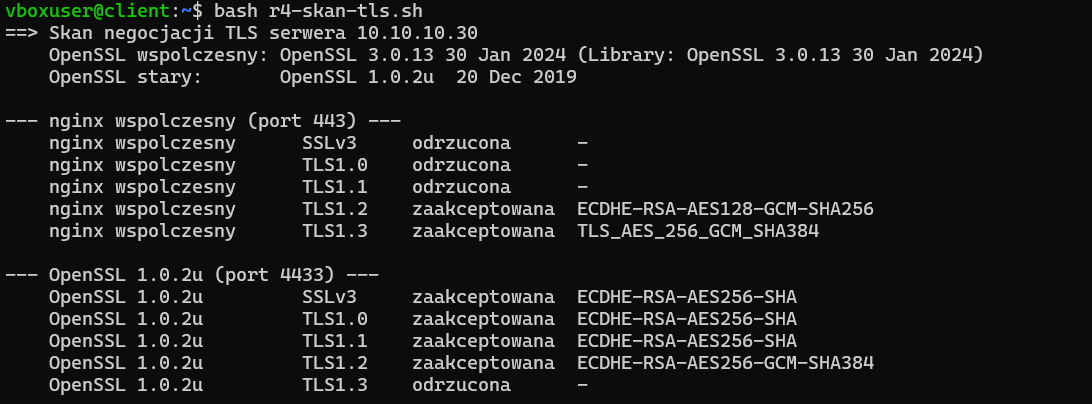
\includegraphics[width=\textwidth]{rysunki/r4-skan-tls.png}
\caption{Wynik skanu wersji protokołu wykonanego skryptem \kod{r4-skan-tls.sh}}
\label{rys:skan-tls}
\end{figure}

Drugą linią obrony przed obniżeniem wersji jest sygnalizacja \kod{TLS\_FALLBACK\_SCSV} (ang. \ang{Signaling Cipher Suite Value}, SCSV), opisana w~RFC~7507~\cite{rfc7507}. Klient, który ponawia nieudane połączenie w~niższej wersji, dołącza do oferty specjalną wartość. Serwer odrzuca takie połączenie alertem \ang{inappropriate\_fallback} (numer 86), ale tylko wtedy, gdy sam obsługuje wersję wyższą niż zaoferowana. W~ramach skanu sprawdzono reakcję obu serwerów na ofertę TLS~1.2 z~sygnałem SCSV. Serwer utwardzony połączenie odrzucił, ponieważ obsługuje TLS~1.3. Serwer przestarzały połączenie przyjął, co jest jednak zgodne ze standardem: TLS~1.2 jest jego wersją najwyższą, a~zatem test ten nie rozstrzygał, czy serwer obsługuje mechanizm SCSV.

Dlatego wykonano test uzupełniający (skrypt \kod{r4-scsv.sh}), w~którym serwerowi przestarzałemu zaoferowano wersje niższe od jego maksymalnej -- z~sygnałem SCSV i~bez niego. Wyniki czterech przypadków zawiera tabela~\ref{tab:scsv}, a~wyjście skryptu rysunek~\ref{rys:scsv}.

\begin{table}[htbp]
\centering\small
\begin{tabularx}{\textwidth}{@{}c l l c L@{}}
\toprule
\textbf{Nr} & \textbf{Serwer} & \textbf{Oferowana wersja} & \textbf{SCSV} & \textbf{Wynik} \\
\midrule
1 & przestarzały (:4433) & TLS~1.1 & tak & odrzucone, alert 86 \\
2 & przestarzały (:4433) & TLS~1.0 & tak & odrzucone, alert 86 \\
3 & przestarzały (:4433) & TLS~1.1 & nie & zestawione: TLS~1.1, \kod{ECDHE-RSA-AES256-SHA} \\
4 & utwardzony (:443)    & TLS~1.2 & tak & odrzucone, alert 86 \\
\bottomrule
\end{tabularx}
\caption{Reakcja serwerów na sygnał obniżenia wersji (test uzupełniający)}
\label{tab:scsv}
\end{table}

\begin{figure}[htbp]
\centering
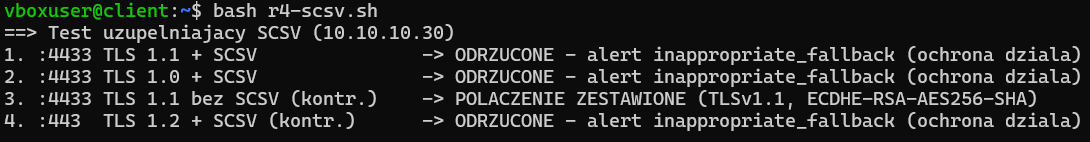
\includegraphics[width=\textwidth]{rysunki/r4-scsv.png}
\caption{Wynik testu uzupełniającego reakcji na sygnał \kod{TLS\_FALLBACK\_SCSV}}
\label{rys:scsv}
\end{figure}

Serwer przestarzały obsługuje mechanizm SCSV poprawnie: odrzucił obie oferty niższych wersji opatrzone sygnałem (przypadki 1 i~2). Ta sama oferta TLS~1.1 bez sygnału (przypadek~3) została jednak przyjęta. Mechanizm SCSV chroni więc wyłącznie klientów, którzy sami sygnalizują obniżenie wersji; klient przestarzały albo skonfigurowany do używania starszej wersji zostanie obsłużony bez zastrzeżeń. Rzeczywistą słabością serwera przestarzałego nie jest zatem brak mechanizmu sygnalizacji, lecz akceptowanie wersji SSLv3, TLS~1.0 i~TLS~1.1. Skuteczną ochroną okazało się dopiero wyłączenie tych wersji po stronie serwera, jak w~konfiguracji utwardzonej. Ruch z~opisanych połączeń zarejestrowany przez czujnik wykorzystano w~podrozdziale~\ref{sec:ids} do oceny reguł wykrywających przestarzałe parametry sesji.

% ---------------------------------------------------------------------
\section{Modyfikacja ciasteczka szyfrowanego w~trybie CTR}\label{sec:ctr}

Eksperymenty z~podrozdziałów~\ref{sec:ctr} i~\ref{sec:cbc} dotyczą ciasteczka sesyjnego aplikacji testowej, które w~zaszyfrowanej postaci przechowuje tekst \kod{user=student;admin=0;uid=1001} (29~bajtów). Pole \kod{admin} decyduje o~dostępie do funkcji administracyjnych. Budowę tokenu w~poszczególnych wariantach przedstawiono w~tabeli~\ref{tab:tokeny}.

\begin{table}[htbp]
\centering\small
\begin{tabularx}{\textwidth}{@{}l L c@{}}
\toprule
\textbf{Wariant} & \textbf{Budowa tokenu (przed kodowaniem Base64)} & \textbf{Długość} \\
\midrule
AES-128-CTR & licznik początkowy (8~B) + kryptogram (29~B) & 37~B \\
AES-128-CBC & wektor inicjujący (16~B) + kryptogram (2 bloki po 16~B, w~tym 3~B dopełnienia) & 48~B \\
AES-128-GCM & wartość jednorazowa (12~B) + kryptogram (29~B) + znacznik uwierzytelniający (16~B) & 57~B \\
\bottomrule
\end{tabularx}
\caption{Budowa tokenu ciasteczka sesyjnego w~badanych wariantach}
\label{tab:tokeny}
\end{table}

\subsection*{Przebieg pomiaru}

Pomiar wykonał skrypt \kod{r4-pomiar-integralnosci.py} uruchomiony na maszynie klienta. Skrypt logował się do aplikacji jako użytkownik \kod{student}, otrzymywał ciasteczko, a~następnie wykonywał dwa rodzaje prób:
\begin{itemize}
  \item \textbf{seria losowa} -- 200~prób dla każdego wariantu; w~każdej próbie zmieniano jeden bajt tokenu na losowej pozycji (operacja XOR z~losową wartością od 1 do 255), wysyłano zmodyfikowane ciasteczko do aplikacji i~zapisywano kod odpowiedzi HTTP oraz to, czy odczytana przez aplikację treść różniła się od pierwotnej;
  \item \textbf{próba celowana} -- zmiana wartości pola \kod{admin} z~0 na 1 przy założeniu, że struktura tekstu jawnego jest znana (typowe założenie o~napastniku, który sam może utworzyć konto w~aplikacji).
\end{itemize}
Modyfikację uznawano za przyjętą, jeżeli aplikacja odpowiedziała kodem 200. Generator liczb pseudolosowych inicjowano stałym ziarnem 20261025, dlatego serię można dokładnie powtórzyć.

\subsection*{Wyniki}

Wyniki serii losowej zawiera tabela~\ref{tab:ctr}. Wariant bez uwierzytelnienia przyjął wszystkie 200~zmodyfikowanych tokenów, a~w~każdym przypadku odczytana treść różniła się od pierwotnej. Wariant GCM odrzucił wszystkie modyfikacje kodem 403, niezależnie od tego, czy zmieniony bajt należał do wartości jednorazowej, kryptogramu, czy znacznika uwierzytelniającego.

\begin{table}[htbp]
\centering\small
\begin{tabularx}{\textwidth}{@{}L rrrrc@{}}
\toprule
\textbf{Wariant} & \textbf{Próby} & \textbf{Przyjęte} & \textbf{Odsetek} & \textbf{Zmieniona treść} & \textbf{Kod odrzucenia} \\
\midrule
AES-128-CTR bez uwierzytelnienia & 200 & 200 & 100\% & 200 & -- \\
AES-128-GCM                      & 200 &   0 &   0\% &   0 & 403 \\
\bottomrule
\end{tabularx}
\caption{Seria losowa modyfikacji ciasteczka -- szyfr strumieniowy}
\label{tab:ctr}
\end{table}

Rozkład prób według pozycji zmienionego bajtu przedstawia górna część rysunku~\ref{rys:pozycje}. Wszystkie pozycje tokenu dały ten sam wynik. Zmiana bajtu kryptogramu (pozycje 8--36) zmienia dokładnie jeden bajt tekstu jawnego. Zmiana licznika początkowego (pozycje 0--7) zmienia cały strumień klucza i~w~efekcie cały odczytany tekst, ale również taki token został przyjęty -- aplikacja nie ma żadnej możliwości odróżnienia go od poprawnego.

\begin{figure}[htbp]
\centering
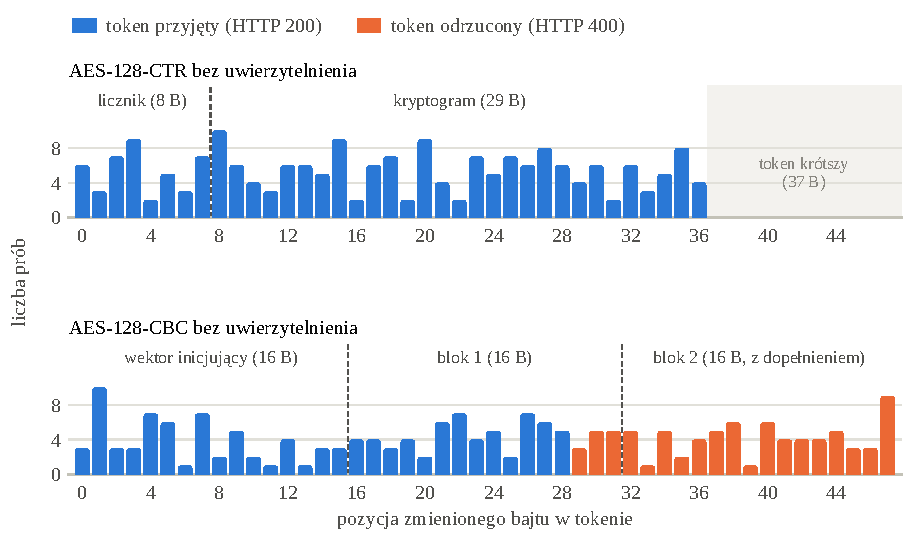
\includegraphics[width=\textwidth]{rysunki/r4-pozycje.pdf}
\caption{Wynik serii losowej w~zależności od pozycji zmienionego bajtu tokenu}
\label{rys:pozycje}
\end{figure}

Wyniki próby celowanej zawiera tabela~\ref{tab:celowane}. W~wariancie CTR zmiana jednego bajtu kryptogramu (pozycja 27, odpowiadająca wartości pola \kod{admin}) dała dokładnie zamierzony efekt: aplikacja odczytała \kod{admin=1}, pozostałe pola pozostały nienaruszone, a~użytkownik uzyskał dostęp do funkcji administracyjnych. W~wariancie GCM analogiczna zmiana została odrzucona.

\begin{table}[htbp]
\centering\small
\begin{tabularx}{\textwidth}{@{}l c c L c@{}}
\toprule
\textbf{Wariant} & \textbf{Pozycja bajtu} & \textbf{HTTP} & \textbf{Pola odczytane przez aplikację} & \textbf{Uprawnienia} \\
\midrule
AES-128-CTR & 27 & 200 & \kod{user=student}, \kod{admin=1}, \kod{uid=1001} & uzyskane \\
AES-128-CBC & 19 & 200 & \kod{uid=1001}; nazwa pola \kod{admin} zniekształcona, pole \kod{user} utracone & nie \\
AES-128-GCM & 31 & 403 & -- (token odrzucony) & nie \\
\bottomrule
\end{tabularx}
\caption{Próba celowana: zmiana wartości pola \kod{admin} z~0 na 1}
\label{tab:celowane}
\end{table}

% ---------------------------------------------------------------------
\section{Modyfikacja ciasteczka szyfrowanego w~trybie CBC}\label{sec:cbc}

Pomiar dla trybu CBC przeprowadzono tym samym skryptem, z~tymi samymi parametrami i~tym samym ziarnem co w~podrozdziale~\ref{sec:ctr}. Wariantem poprawionym był ponownie tryb GCM, dla którego wykonano osobną serię 200~prób.

\subsection*{Wyniki}

Wariant CBC bez uwierzytelnienia przyjął 120 z~200~zmodyfikowanych tokenów (60\%), a~każdy przyjęty token miał zmienioną treść (tabela~\ref{tab:cbc}). Odrzucone tokeny aplikacja odrzucała kodem 400, sygnalizującym błąd odczytu ciasteczka. Wariant GCM ponownie odrzucił wszystkie modyfikacje.

\begin{table}[htbp]
\centering\small
\begin{tabularx}{\textwidth}{@{}L rrrrc@{}}
\toprule
\textbf{Wariant} & \textbf{Próby} & \textbf{Przyjęte} & \textbf{Odsetek} & \textbf{Zmieniona treść} & \textbf{Kod odrzucenia} \\
\midrule
AES-128-CBC bez uwierzytelnienia & 200 & 120 & 60\% & 120 & 400 \\
AES-128-GCM                      & 200 &   0 &  0\% &   0 & 403 \\
\bottomrule
\end{tabularx}
\caption{Seria losowa modyfikacji ciasteczka -- szyfr blokowy}
\label{tab:cbc}
\end{table}

W~odróżnieniu od trybu CTR wynik zależał od miejsca modyfikacji (dolna część rysunku~\ref{rys:pozycje}). Wszystkie modyfikacje wektora inicjującego zostały przyjęte, modyfikacje pierwszego bloku kryptogramu -- prawie wszystkie, a~modyfikacje drugiego bloku -- żadna. Odrzucenia w~pierwszym bloku wystąpiły wyłącznie na pozycjach 29--31. Rozkład ten można przewidzieć na podstawie budowy tokenu (tabela~\ref{tab:tokeny}):
\begin{itemize}
  \item zmiana wektora inicjującego zmienia jeden bajt pierwszego bloku tekstu jawnego i~nie dotyka dopełnienia, więc token zawsze zostaje przyjęty;
  \item zmiana pierwszego bloku kryptogramu zniekształca cały pierwszy blok tekstu jawnego i~zmienia jeden bajt drugiego bloku na tej samej pozycji; token zostaje odrzucony tylko wtedy, gdy zmiana trafi w~jeden z~3~bajtów dopełnienia (pozycje 29--31), co daje oczekiwany odsetek przyjęć $13/16 = 81{,}25\%$;
  \item zmiana drugiego bloku kryptogramu zniekształca cały ostatni blok tekstu jawnego razem z~dopełnieniem; token zostanie przyjęty tylko wtedy, gdy losowy wynik przypadkiem utworzy poprawne dopełnienie, czyli z~prawdopodobieństwem około $1/256$.
\end{itemize}

Porównanie wartości zmierzonych z~oczekiwanymi zawiera tabela~\ref{tab:cbc-obszary} i~rysunek~\ref{rys:cbc-obszary}. Oczekiwany odsetek dla całej serii, ważony liczbą prób w~poszczególnych obszarach, wynosi 59,9\%, a~zmierzony 60,0\%. Zgodność ta potwierdza, że o~przyjęciu zmodyfikowanego tokenu decydowała wyłącznie poprawność dopełnienia, a~sama aplikacja nie wykrywała modyfikacji treści.

\begin{table}[htbp]
\centering\small
\begin{tabular}{@{}llrrrr@{}}
\toprule
\textbf{Obszar tokenu} & \textbf{Pozycje} & \textbf{Próby} & \textbf{Przyjęte} & \textbf{Odsetek} & \textbf{Oczekiwany} \\
\midrule
wektor inicjujący        & 0--15  &  61 &  61 & 100,0\% & 100,0\% \\
pierwszy blok kryptogramu & 16--31 &  72 &  59 &  81,9\% &  81,25\% \\
drugi blok kryptogramu    & 32--47 &  67 &   0 &   0,0\% &  $\approx 0{,}4\%$ \\
\midrule
\textbf{Razem}           & 0--47  & 200 & 120 &  60,0\% &  59,9\% \\
\bottomrule
\end{tabular}
\caption{Wariant CBC: odsetek przyjętych modyfikacji według obszaru tokenu}
\label{tab:cbc-obszary}
\end{table}

\begin{figure}[htbp]
\centering
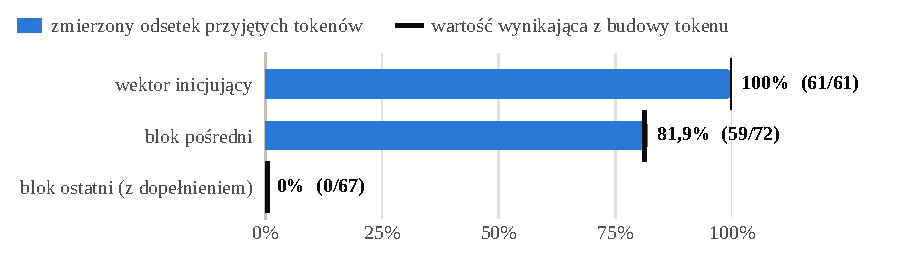
\includegraphics[width=\textwidth]{rysunki/r4-cbc-obszary.pdf}
\caption{Wariant CBC: zmierzony odsetek przyjętych tokenów na tle wartości wynikającej z~budowy tokenu}
\label{rys:cbc-obszary}
\end{figure}

Próba celowana w~trybie CBC nie dała napastnikowi uprawnień (tabela~\ref{tab:celowane}). Wartość pola \kod{admin} znajduje się w~drugim bloku tekstu jawnego (bajt 19), więc jej zmiana wymaga modyfikacji pierwszego bloku kryptogramu, która zniekształca cały pierwszy blok tekstu jawnego -- \kod{user=student;adm}. Aplikacja odczytała wprawdzie wartość~1, ale pod zniekształconą nazwą pola, przez co nie rozpoznała jej jako pola \kod{admin}. O~niepowodzeniu zdecydował więc układ danych w~blokach, a~nie właściwość trybu: gdyby modyfikowane pole leżało w~pierwszym bloku, zmianę można by przeprowadzić przez wektor inicjujący, którego modyfikacje były przyjmowane w~100\% przypadków i~nie zniekształcały pozostałych danych.

Pomiar ujawnił też dodatkową słabość wariantu podatnego: aplikacja odpowiadała innym kodem na błąd dopełnienia (400) niż na pozostałe błędy weryfikacji. Rozróżnialne komunikaty o~błędzie dopełnienia ujawniają informację o~poprawności odszyfrowanych danych i~w~przeszłości stanowiły podstawę skutecznych ataków na tryb CBC~\cite{boneh2023}. Niezależnie od zmiany trybu szyfrowania zaleca się więc zwracanie jednakowej odpowiedzi dla wszystkich błędów odczytu ciasteczka.

% ---------------------------------------------------------------------
\section{Weryfikacja podpisu żądań: SHA-256(sekret~$\|$~wiadomość) a~HMAC}\label{sec:lenext}

Aplikacja testowa uwierzytelnia żądania API podpisem dołączanym do treści żądania. W~wariancie podatnym podpis to skrót SHA-256 z~połączenia sekretu i~wiadomości, a~w~wariancie poprawionym -- kod HMAC-SHA-256 (tabela~\ref{tab:aplikacja}). Oba warianty korzystają z~tego samego 16-bajtowego sekretu, losowanego przy starcie aplikacji.

\subsection*{Przebieg pomiaru}

Skrypt \kod{r4-pomiar-integralnosci.py} pobierał z~aplikacji poprawnie podpisane żądanie przelewu, a~następnie wysyłał do każdego wariantu pięć jego odmian: żądanie nienaruszone, żądanie ze zmienioną wartością pola, żądanie z~doklejonym na końcu dodatkowym polem (bez zmiany podpisu), żądanie ze zmienionym jednym znakiem podpisu oraz żądanie z~podpisem losowym. Dla każdej odmiany zapisywano kod odpowiedzi HTTP.

\subsection*{Wyniki}

Wyniki zestawiono w~tabeli~\ref{tab:podpis}. Oba warianty przyjęły wyłącznie żądanie nienaruszone, a~wszystkie cztery naruszenia pary (wiadomość, podpis) odrzuciły kodem 403. Weryfikacja podpisu jest więc w~obu wariantach zaimplementowana poprawnie i~test czarnoskrzynkowy nie odróżnia od siebie obu konstrukcji.

\begin{table}[htbp]
\centering\small
\begin{tabular}{@{}lcc@{}}
\toprule
\textbf{Przypadek} & \textbf{SHA-256(sekret~$\|$~wiadomość)} & \textbf{HMAC-SHA-256} \\
\midrule
żądanie nienaruszone                    & 200 -- przyjęte   & 200 -- przyjęte \\
zmieniona wartość pola                  & 403 -- odrzucone  & 403 -- odrzucone \\
doklejone pole, podpis bez zmian        & 403 -- odrzucone  & 403 -- odrzucone \\
zmieniony jeden znak podpisu            & 403 -- odrzucone  & 403 -- odrzucone \\
podpis losowy                           & 403 -- odrzucone  & 403 -- odrzucone \\
\bottomrule
\end{tabular}
\caption{Reakcja aplikacji na naruszenie pary (wiadomość, podpis)}
\label{tab:podpis}
\end{table}

Różnica między wariantami wynika z~budowy funkcji skrótu, a~nie z~implementacji weryfikacji. Funkcja SHA-256 ma konstrukcję Merkle'a--Damgårda, w~której wynik jest stanem wewnętrznym po przetworzeniu ostatniego bloku danych. Znając podpis $\mathrm{SHA\text{-}256}(s \| m)$ oraz długość sekretu, można więc obliczyć poprawny podpis dla wiadomości przedłużonej o~dopełnienie i~dowolny sufiks, nie znając sekretu (atak przedłużenia, ang. \ang{length extension}). Konstrukcja HMAC przetwarza wynik wewnętrznego skrótu drugi raz, z~innym kluczem, i~tej własności nie ma (podrozdział~\ref{sec:skroty})~\cite{boneh2023}. Przypadek z~doklejonym polem odrzucono w~obu wariantach, ponieważ nie zmieniono podpisu; pomiar nie obejmował obliczania podpisu dla wiadomości przedłużonej. Podatność wariantu z~konstrukcją $\mathrm{SHA\text{-}256}(s \| m)$ wynika więc z~analizy konstrukcji, a~pomiar potwierdza jedynie, że pozostałe elementy weryfikacji działają w~obu wariantach tak samo.

% ---------------------------------------------------------------------
\section{Podsumowanie wyników}\label{sec:ataki-podsum}

Odsetek przyjętych zmodyfikowanych ciasteczek w~trzech badanych trybach szyfrowania zestawiono na rysunku~\ref{rys:odsetek}, a~wyniki wszystkich eksperymentów rozdziału -- w~tabeli~\ref{tab:r4-podsum}.

\begin{figure}[htbp]
\centering
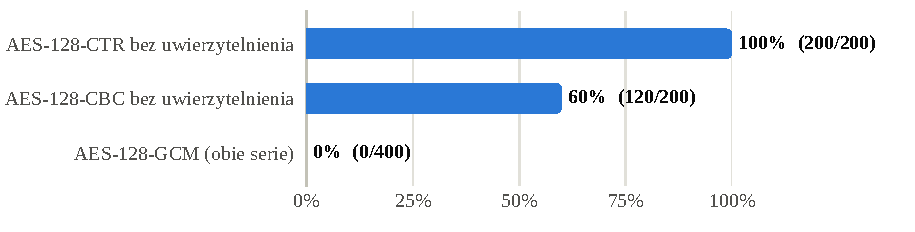
\includegraphics[width=\textwidth]{rysunki/r4-odsetek.pdf}
\caption{Odsetek przyjętych zmodyfikowanych ciasteczek w~seriach losowych}
\label{rys:odsetek}
\end{figure}

\begin{table}[htbp]
\centering\small
\begin{tabularx}{\textwidth}{@{}>{\raggedright\arraybackslash}p{2.6cm} L L@{}}
\toprule
\textbf{Mechanizm} & \textbf{Wariant podatny -- wynik} & \textbf{Wariant poprawiony -- wynik} \\
\midrule
podszycie w~ARP & -- & inspektor \kod{arp\_spoof}: 3 z~3 ramek wykryte (6~alarmów), 0~alarmów dla ogłoszeń poprawnych \\
negocjacja TLS & OpenSSL 1.0.2u: 4 z~5 wersji, w~tym SSLv3; SCSV działa tylko dla klienta, który go wyśle & nginx: wyłącznie TLS~1.2 i~1.3 z~zestawami AEAD; SCSV działa \\
ciasteczko, szyfr strumieniowy & AES-CTR: 100\% modyfikacji przyjętych, uprawnienia administratora uzyskane & AES-GCM: 0\% przyjętych \\
ciasteczko, szyfr blokowy & AES-CBC: 60\% przyjętych, zgodnie z~modelem (59,9\%); próba celowana nieudana z~powodu układu danych & AES-GCM: 0\% przyjętych \\
podpis żądania & SHA-256(sekret~$\|$~wiadomość): naruszenia odrzucone, konstrukcja podatna na atak przedłużenia & HMAC-SHA-256: naruszenia odrzucone, konstrukcja odporna \\
\bottomrule
\end{tabularx}
\caption{Zestawienie wyników rozdziału~\ref{ch:ataki}}
\label{tab:r4-podsum}
\end{table}

Z~przeprowadzonych eksperymentów wynikają następujące wnioski:
\begin{enumerate}
  \item \textbf{Poufność nie zapewnia integralności.} Oba tryby bez uwierzytelnienia przyjmowały zmodyfikowane dane, mimo że napastnik nie znał klucza. Tryb GCM odrzucił wszystkie 400~modyfikacji w~obu seriach.
  \item \textbf{Podatność zależy od budowy trybu.} W~trybie CTR każda zmiana została przyjęta, a~zmiana celowana dała dokładnie zamierzony efekt. W~trybie CBC skutek zależał od położenia zmiany, a~zmierzony rozkład zgadzał się z~wartością wynikającą z~budowy tokenu z~dokładnością do 0,1~punktu procentowego.
  \item \textbf{Ochrona przed obniżeniem wersji musi być po stronie serwera.} Mechanizm SCSV działa tylko wtedy, gdy klient sam zasygnalizuje ponowienie połączenia. Pewną ochronę daje dopiero wyłączenie wersji starszych niż TLS~1.2.
  \item \textbf{Próby ataku pozostawiają ślad w~ruchu sieciowym.} Zarówno podszycie w~ARP, jak i~zestawienie sesji z~przestarzałymi parametrami są widoczne dla czujnika. Na tej obserwacji oparto warstwę detekcji sieciowej opisaną w~rozdziale~\ref{ch:obrona}.
\end{enumerate}

% =====================================================================
%  Rozdział 5 - wersja robocza do przeredagowania
%  Dane: wyniki/E4 (22-24.10.2026, powtórka Argon2 1 GiB 8.11.2026)
%  Wszystkie liczby zweryfikowane z plików podsumowań w repozytorium.
%  Wykresy: tools/wykresy-praca.py r5
% =====================================================================
\chapter{Badanie wydajności kryptoanalizy offline z~wykorzystaniem GPU}\label{ch:gpu}

W rozdziale przedstawiono pomiary szybkości, z~jaką konsumencka karta graficzna sprawdza kandydatów na hasło chroniące zaszyfrowane pliki. Rozważany jest atak offline, w~którym napastnik dysponuje kopią pliku i~sprawdza kolejne hasła bez ograniczeń narzucanych przez usługę sieciową. Jedyną przeszkodą jest wtedy koszt obliczeniowy funkcji wyprowadzania klucza z~hasła (ang. \ang{key derivation function}, KDF), omówionej w~podrozdziale~\ref{sec:kdf}. Celem pomiarów było wyznaczenie tego kosztu dla funkcji różnego typu, zbadanie jego zależności od parametrów oraz sprawdzenie, czy funkcje wymagające dużej ilości pamięci (ang. \ang{memory-hard}) rzeczywiście ograniczają przewagę karty graficznej nad procesorem. Pomiary mierzą wyłącznie przepustowość sprawdzania kandydatów; nie dotyczą odtworzenia żadnego rzeczywistego hasła, a~ich wynikiem jest koszt, jaki zabezpieczenie narzuca atakującemu.

% ---------------------------------------------------------------------
\section{Zakres i~plan eksperymentu}\label{sec:gpu-plan}

Pomiary wykonano na platformie opisanej w~podrozdziale~\ref{sec:platforma}: karta NVIDIA GeForce GTX~1660 (6~GB), procesor AMD Ryzen~5~5600, program Hashcat 7.1.2. Maszyny wirtualne laboratorium pozostawały w~tym czasie wyłączone, aby nie obciążały platformy. Zaplanowano cztery serie pomiarów (tabela~\ref{tab:r5-pomiary}).

\begin{table}[htbp]
\centering\small
\begin{tabularx}{\textwidth}{@{}c >{\raggedright\arraybackslash}p{3.5cm} L c c@{}}
\toprule
\textbf{Seria} & \textbf{Zakres} & \textbf{Sposób pomiaru} & \textbf{Powt.} & \textbf{Data} \\
\midrule
1 & 6~formatów, GPU & wbudowany test wydajności (\kod{-b}) na wzorcowych próbkach & 3 + 3 & 22, 23.10 \\
2 & własne pliki, GPU & pomiar przepustowości przez 40~s: VeraCrypt z~trzema wartościami PIM, 7-Zip, KeePass AES-KDF & 3 & 24.10 \\
3 & 5~formatów, GPU i~CPU & test \kod{-b} osobno na obu urządzeniach & 2 & 24.10 \\
4 & Argon2id 64, 256, 1024~MiB; GPU i~CPU & pomiar przepustowości przez 40--60~s & 2 / 3 & 24.10, 8.11 \\
\bottomrule
\end{tabularx}
\caption{Serie pomiarów wydajności kryptoanalizy}
\label{tab:r5-pomiary}
\end{table}

Pliki testowe utworzono tak, aby dwa pliki tego samego rodzaju różniły się tylko jednym parametrem (tabela~\ref{tab:r5-pliki}). Pozwala to przypisać zmianę wyniku jednej przyczynie. Bazy KeePass w~formacie KDBX~4 z~funkcją Argon2 przygotowano, ale nie udało się ich użyć: narzędzie wyodrębniające materiał do analizy obsługuje jedynie starszy format KDBX~3.1 i~dla formatu KDBX~4 zgłaszało błąd nieznanej wersji. Z~tego powodu wpływ pamięci funkcji Argon2 zbadano w~serii~4 na skrótach Argon2id wygenerowanych biblioteką \kod{argon2-cffi}, różniących się wyłącznie parametrem pamięci, przy stałych parametrach czasu $t = 3$ i~równoległości $p = 1$. Zestaw ten odpowiada drugiemu z~wariantów zalecanych w~RFC~9106~\cite{rfc9106}.

\begin{table}[htbp]
\centering\small
\begin{tabularx}{\textwidth}{@{}>{\raggedright\arraybackslash}p{3.1cm} >{\raggedright\arraybackslash}p{3.1cm} L@{}}
\toprule
\textbf{Plik} & \textbf{Funkcja KDF} & \textbf{Parametr kosztu} \\
\midrule
3~kontenery VeraCrypt (AES) & PBKDF2-HMAC-SHA-512 & PIM 1 / 250 / 500, tj. 16\,000 / 265\,000 / 515\,000 iteracji \\
archiwum 7-Zip (AES-256) & SHA-256 iterowane & $2^{19}$ iteracji, z~weryfikacją danych archiwum \\
baza KeePass KDBX~3.1 (AES) & AES-KDF & 100\,000 rund \\
3~bazy KeePass KDBX~4 (AES) & Argon2d & 64 / 256 / 1024~MiB (nieużyte) \\
3~skróty Argon2id & Argon2id & 64 / 256 / 1024~MiB, $t = 3$, $p = 1$ \\
\bottomrule
\end{tabularx}
\caption{Pliki i~skróty testowe; kolejne pliki tego samego rodzaju różnią się jednym parametrem}
\label{tab:r5-pliki}
\end{table}

Przepustowość mierzono dwiema metodami. W~seriach~1 i~3 użyto wbudowanego testu wydajności programu (\kod{-b}), który podaje liczbę sprawdzeń na sekundę dla skrótu wzorcowego. W~seriach~2 i~4 program sprawdzał kandydatów z~ustalonej przestrzeni przez zadany czas, a~jako wynik przyjęto liczbę kandydatów podzieloną przez czas. W~seriach~2 i~4 nie dążono do odgadnięcia hasła, lecz jedynie do zmierzenia tempa sprawdzania; przestrzeń kandydatów dobrano tak, aby żaden z~nich nie był właściwym hasłem. Każdy pomiar powtarzano (tabela~\ref{tab:r5-pomiary}) i~podawano wartość średnią. Dla funkcji najwolniejszych, gdzie tempo spada do pojedynczych sprawdzeń na sekundę, zaokrąglany odczyt programu jest zbyt zgrubny, więc tempo wyznaczano z~przyrostu licznika postępu między dwoma odczytami stanu.

Aby wykluczyć wpływ nagrzania karty na wyniki, w~czasie części pomiarów rejestrowano co około 2~s jej temperaturę, taktowanie i~pobór mocy. Przebieg dla najdłuższej serii (VeraCrypt, seria~2) przedstawia rysunek~\ref{rys:karta}. Pod pełnym obciążeniem temperatura rdzenia nie przekroczyła 66~$^\circ$C, a~taktowanie rdzeni utrzymywało się w~przedziale 1920--1980~MHz bez tendencji spadkowej. Temperatura pozostawała więc znacznie poniżej progu obniżania taktowania, a~karta nie ograniczała wydajności w~trakcie pomiaru. Rozrzut między powtórzeniami nie przekraczał 1\% dla wszystkich funkcji poza 7-Zip (5,8\%, co wyjaśniono w~podrozdziale~\ref{sec:gpu-compute}), co potwierdza powtarzalność warunków.

\begin{figure}[htbp]
\centering
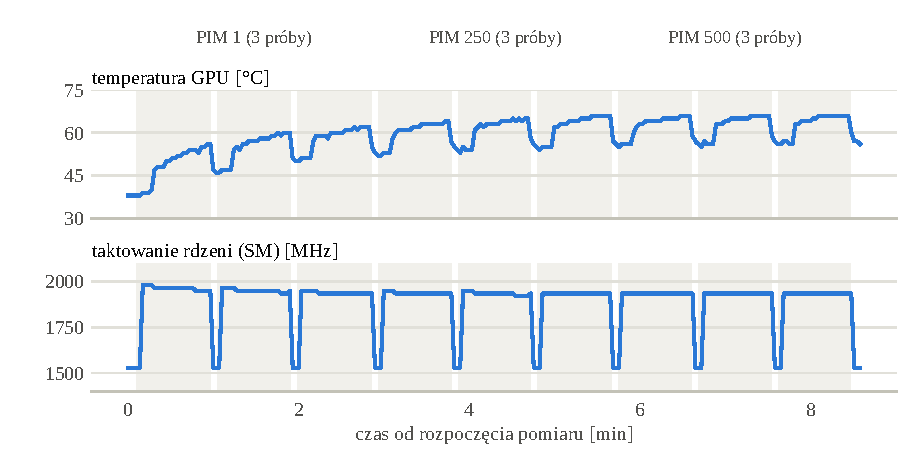
\includegraphics[width=\textwidth]{rysunki/r5-karta.pdf}
\caption{Temperatura i~taktowanie karty w~trakcie serii pomiarów VeraCrypt; szarym tłem oznaczono okresy obciążenia}
\label{rys:karta}
\end{figure}

% ---------------------------------------------------------------------
\section{Wyniki dla algorytmów compute-hard}\label{sec:gpu-compute}

Pierwszą serię pomiarów wykonano wbudowanym testem wydajności dla sześciu formatów, od szybkich funkcji skrótu po funkcje wyprowadzania klucza (tabela~\ref{tab:r5-benchmark}). Różnice sięgają ośmiu rzędów wielkości: szybkie funkcje skrótu MD5 i~NTLM osiągają dziesiątki miliardów sprawdzeń na sekundę, podczas gdy funkcje KDF spowalniają atak od czterech (7-Zip) do ponad siedmiu (Argon2) rzędów wielkości względem MD5. Rozkład prędkości na skali logarytmicznej przedstawia rysunek~\ref{rys:predkosci}. Potwierdza to, że sama szybka funkcja skrótu nie nadaje się do ochrony haseł, a~właściwą barierą dla atakującego jest dopiero funkcja KDF o~odpowiednim koszcie.

\begin{table}[htbp]
\centering\small
\begin{tabular}{@{}llrr@{}}
\toprule
\textbf{Funkcja} & \textbf{Typ} & \textbf{Prędkość GPU [H/s]} & \textbf{Spowolnienie} \\
\midrule
MD5                        & szybka funkcja skrótu & 20\,070\,400\,000 & 1$\times$ \\
NTLM                       & szybka funkcja skrótu & 34\,954\,233\,333 & 0,57$\times$ \\
7-Zip (SHA-256)            & compute-hard & 309\,633 & 64\,820$\times$ \\
KeePass AES-KDF (KDBX~3.1) & compute-hard & 19\,638 & 1\,022\,001$\times$ \\
VeraCrypt (PBKDF2-SHA-512) & compute-hard & 782 & 25\,654\,538$\times$ \\
KeePass Argon2 (KDBX~4)    & memory-hard  & 460 & 43\,599\,710$\times$ \\
\bottomrule
\end{tabular}
\caption{Wbudowany test wydajności: prędkość na GPU i~krotność spowolnienia względem MD5 (wartość poniżej~1 oznacza funkcję szybszą niż MD5)}
\label{tab:r5-benchmark}
\end{table}

\begin{figure}[htbp]
\centering
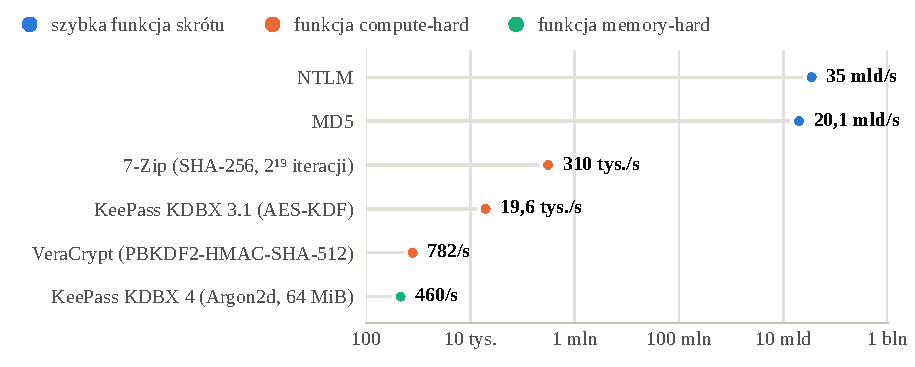
\includegraphics[width=\textwidth]{rysunki/r5-predkosci.pdf}
\caption{Prędkość sprawdzania kandydatów na GPU dla sześciu formatów (skala logarytmiczna)}
\label{rys:predkosci}
\end{figure}

Wbudowany test posługuje się jednak wzorcowymi skrótami o~parametrach dobranych przez autorów narzędzia, które nie muszą odpowiadać plikom spotykanym w~praktyce. Dlatego dwie funkcje compute-hard zmierzono dodatkowo na własnych plikach o~znanych parametrach (tabela~\ref{tab:r5-wlasne}). W~obu przypadkach prędkość okazała się niższa niż w~teście wbudowanym. Dla KeePass AES-KDF stosunek $19\,638 / 4\,734 \approx 4{,}1$ odpowiada liczbie 100\,000~rund w~pliku testowym, większej niż w~skrócie wzorcowym. Dla 7-Zip różnica jest znacznie większa, ponieważ przy rzeczywistym archiwum program musi dla każdego kandydata odszyfrować i~zweryfikować właściwe dane, a~nie tylko sprawdzić krótki wzorzec; stąd także wyższy rozrzut wyników (5,8\%), zależny od zawartości archiwum. Wynika z~tego, że wbudowany test zawyża prędkość atakującego względem realnych plików z~poprawnie dobranym kosztem, a~rzetelna ocena bezpieczeństwa wymaga pomiaru na plikach o~znanych parametrach.

\begin{table}[htbp]
\centering\small
\begin{tabularx}{\textwidth}{@{}L >{\raggedright\arraybackslash}p{3.4cm} r r r@{}}
\toprule
\textbf{Plik} & \textbf{Parametr kosztu} & \textbf{GPU [H/s]} & \textbf{Rozrzut} & \textbf{Test \kod{-b} [H/s]} \\
\midrule
archiwum 7-Zip (AES-256) & $2^{19}$ iteracji SHA-256, weryfikacja danych & 6\,735 & 5,8\% & 309\,633 \\
baza KeePass AES-KDF (KDBX~3.1) & 100\,000 rund & 4\,734 & 0,5\% & 19\,638 \\
\bottomrule
\end{tabularx}
\caption{Pomiar na własnych plikach compute-hard w~zestawieniu z~testem wbudowanym}
\label{tab:r5-wlasne}
\end{table}

% ---------------------------------------------------------------------
\section{Wpływ parametrów kosztu na wydajność}\label{sec:gpu-koszt}

Funkcje compute-hard pozwalają dobrać koszt ataku przez liczbę iteracji. Zależność tę zmierzono na trzech kontenerach VeraCrypt różniących się wyłącznie parametrem PIM, który steruje liczbą iteracji PBKDF2 według wzoru $15\,000 + \text{PIM} \times 1\,000$. Wyniki zawiera tabela~\ref{tab:r5-pim}, a~ich przebieg -- rysunek~\ref{rys:pim}.

\begin{table}[htbp]
\centering\small
\begin{tabular}{@{}rrrrr@{}}
\toprule
\textbf{PIM} & \textbf{Iteracje} & \textbf{Prędkość [H/s]} & \textbf{Rozrzut} & \textbf{Prędkość $\times$ iteracje} \\
\midrule
1   & 16\,000  & 20\,590,7 & 0,6\% & 329,5~mln \\
250 & 265\,000 & 1\,278,3  & 0,0\% & 338,7~mln \\
500 & 515\,000 & 659,0     & 0,0\% & 339,4~mln \\
\bottomrule
\end{tabular}
\caption{VeraCrypt: wpływ liczby iteracji PBKDF2 (parametr PIM) na prędkość ataku}
\label{tab:r5-pim}
\end{table}

\begin{figure}[htbp]
\centering
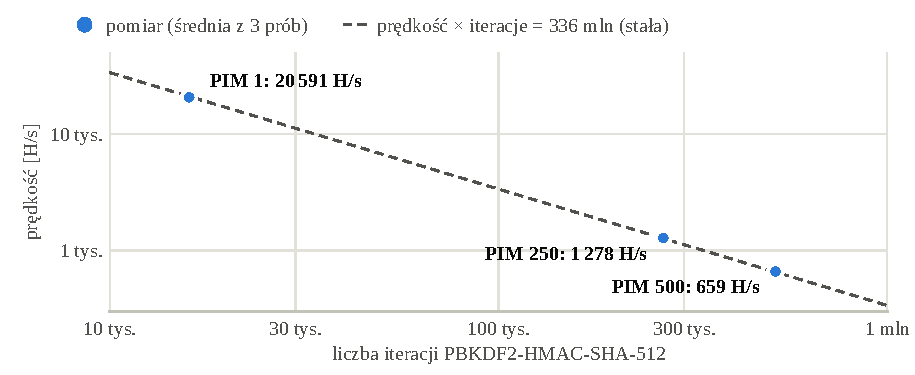
\includegraphics[width=\textwidth]{rysunki/r5-pim.pdf}
\caption{VeraCrypt: prędkość ataku w~funkcji liczby iteracji (skala logarytmiczna na obu osiach)}
\label{rys:pim}
\end{figure}

Prędkość jest odwrotnie proporcjonalna do liczby iteracji: iloczyn prędkości i~liczby iteracji pozostaje niemal stały (329--339~mln), a~przy 32-krotnym wzroście liczby iteracji (z~16\,000 do~515\,000) prędkość spada około 31-krotnie (z~20\,591 do~659~H/s). Parametr kosztu przekłada się więc niemal liniowo na nakład pracy atakującego, co pozwala obrońcy dobrać go do dostępnej mocy obliczeniowej przeciwnika. Nieco niższy iloczyn dla PIM~1 wynika ze stałego narzutu na każdego kandydata (uruchomienie jądra obliczeniowego, odczyt kontenera), który przy małej liczbie iteracji waży proporcjonalnie więcej. Wartość tę wykorzystano też do wyznaczenia odniesienia na rysunku~\ref{rys:pim} (linia stałego iloczynu, średnio 336~mln).

Ograniczeniem funkcji compute-hard jest to, że koszt jednego sprawdzenia rośnie tak samo dla obrońcy, jak i~dla atakującego, a~atakujący dysponuje zwykle znacznie wydajniejszym sprzętem. Skala tej przewagi sprzętowej jest przedmiotem podrozdziału~\ref{sec:gpu-cpu}.

% ---------------------------------------------------------------------
\section{Wyniki dla algorytmów memory-hard}\label{sec:gpu-memory}

Funkcje memory-hard ograniczają atak w~inny sposób: wymagają, by każde sprawdzenie dysponowało dużym, osobnym blokiem pamięci. Masowa równoległość karty graficznej opiera się na jednoczesnym liczeniu tysięcy kandydatów, a~każdy z~nich potrzebuje wtedy własnego bloku pamięci. Gdy pamięć karty się wyczerpuje, liczba równolegle sprawdzanych kandydatów spada, a~wraz z~nią przewaga karty~\cite{eum2023}. Zależność tę zmierzono dla funkcji Argon2id przy trzech rozmiarach pamięci (64, 256 i~1024~MiB) i~stałych pozostałych parametrach, na GPU i~na CPU (tabela~\ref{tab:r5-argon2}, rysunek~\ref{rys:argon2}).

\begin{table}[htbp]
\centering\small
\begin{tabular}{@{}rrrrr@{}}
\toprule
\textbf{Pamięć Argon2} & \textbf{GPU [H/s]} & \textbf{CPU [H/s]} & \textbf{GPU/CPU} & \textbf{Zrównoleglenie GPU} \\
\midrule
64~MiB  & 288,4 & 34,2 & 8,4$\times$ & 83 \\
256~MiB & 30,0  & 7,65 & 3,9$\times$ & 20 \\
1~GiB   & 1,60  & 0,77 & 2,1$\times$ & 4 \\
\bottomrule
\end{tabular}
\caption{Argon2id: prędkość na GPU i~CPU oraz ich stosunek w~funkcji wymaganej pamięci (kolumna ostatnia -- współczynnik zrównoleglenia dobrany przez Hashcat na GPU)}
\label{tab:r5-argon2}
\end{table}

\begin{figure}[htbp]
\centering
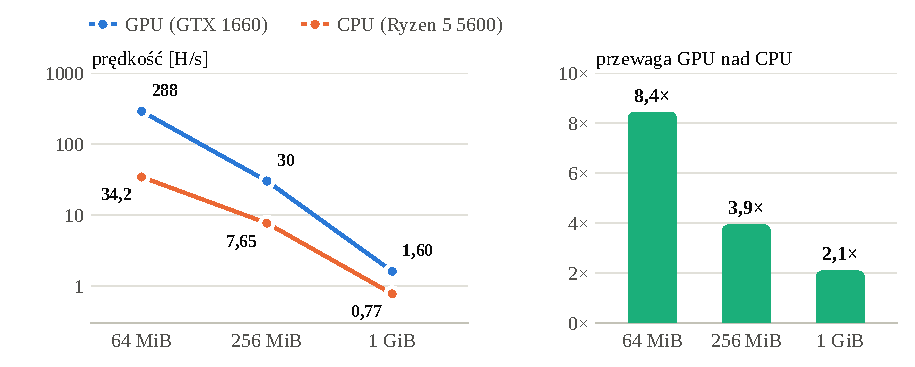
\includegraphics[width=\textwidth]{rysunki/r5-argon2.pdf}
\caption{Argon2id: prędkość na GPU i~CPU (lewy panel) oraz przewaga GPU nad CPU (prawy panel) przy rosnącej pamięci}
\label{rys:argon2}
\end{figure}

Wraz ze wzrostem wymaganej pamięci przewaga GPU nad CPU maleje: z~8,4-krotnej przy 64~MiB, przez 3,9-krotną przy 256~MiB, do 2,1-krotnej przy 1~GiB. Jednocześnie współczynnik zrównoleglenia dobierany przez program na karcie spada z~83 do~4, a~jego iloczyn z~pamięcią pojedynczego sprawdzenia pozostaje rzędu pojemności karty (odpowiednio około 5,2, 5,0 i~4,0~GiB wobec 6~GB karty). Wskazuje to, że liczbę jednocześnie sprawdzanych kandydatów ogranicza nie moc obliczeniowa, lecz pamięć karty -- co jest istotą ochrony, jaką funkcje memory-hard dają przeciwko atakom z~użyciem GPU.

Pomiar dla 1~GiB wykonano jako osobną powtórkę (8.11.2026). We wcześniejszej serii (24.10) przy tym rozmiarze pamięci program kończył się na karcie błędem przydziału bufora i~obliczeń nie wykonywał, podczas gdy powtórka trzykrotnie zakończyła się powodzeniem z~jednakowym wynikiem (rysunek~\ref{rys:argon2-1gib}). Rozbieżność tę przypisano stanowi pamięci karty w~chwili doboru rozmiaru buforów: 1~GiB na pojedyncze sprawdzenie leży na granicy możliwości tej karty, powyżej której przydział bufora bywa odrzucany. W~powtórce program zgłosił ponadto zajęcie około 1,1~GB pamięci karty przez inne procesy i~ograniczył wykorzystanie do 83\%, dlatego zmierzoną prędkość GPU dla 1~GiB należy traktować jako dolne oszacowanie; bez tego ograniczenia stosunek GPU/CPU nie przekroczyłby około 2,5-krotności, co nie zmienia wniosku o~malejącej przewadze karty.

\begin{figure}[htbp]
\centering
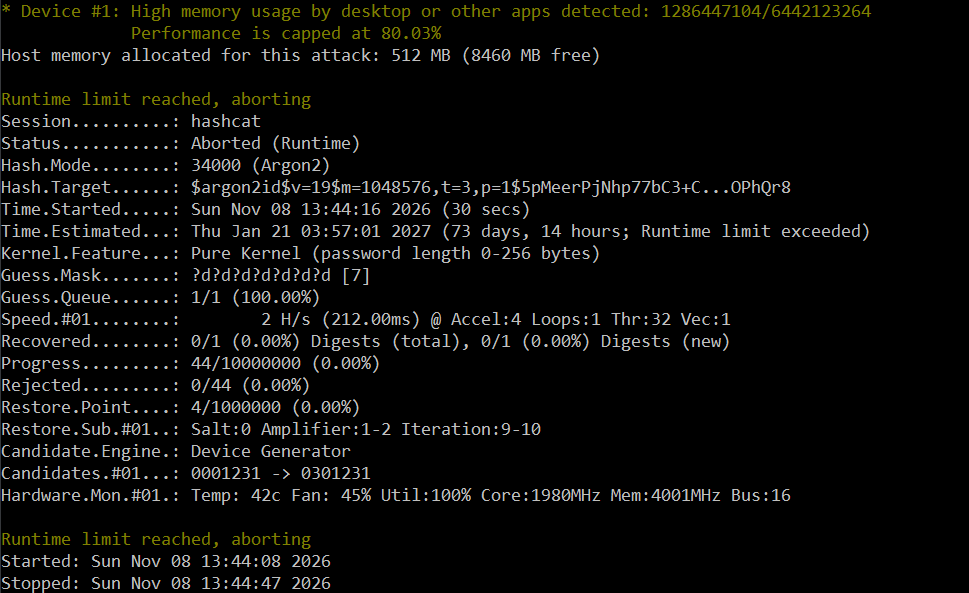
\includegraphics[width=0.85\textwidth]{rysunki/r5-argon2-1gib.png}
\caption{Pomiar Argon2id z~pamięcią 1~GiB na GPU z~widocznym ograniczeniem wykorzystania karty}
\label{rys:argon2-1gib}
\end{figure}

% ---------------------------------------------------------------------
\section{Porównanie GPU i~CPU oraz interpretacja wyników}\label{sec:gpu-cpu}

Przewagę karty graficznej nad procesorem zmierzono osobno dla pięciu funkcji, uruchamiając ten sam test na GPU i~na CPU (tabela~\ref{tab:r5-gpucpu}). Zestawienie wszystkich wyznaczonych stosunków, łącznie z~serią Argon2 z~podrozdziału~\ref{sec:gpu-memory}, przedstawia rysunek~\ref{rys:gpu-cpu}.

\begin{table}[htbp]
\centering\small
\begin{tabular}{@{}lrrr@{}}
\toprule
\textbf{Funkcja} & \textbf{GPU [H/s]} & \textbf{CPU [H/s]} & \textbf{GPU/CPU} \\
\midrule
MD5                         & 20\,016\,200\,000 & 1\,218\,600\,000 & 16,4$\times$ \\
7-Zip (SHA-256)             & 310\,100 & 7\,478 & 41,5$\times$ \\
KeePass AES-KDF             & 19\,794  & 2\,666,5 & 7,4$\times$ \\
VeraCrypt (PBKDF2-SHA-512)  & 786 & 70 & 11,2$\times$ \\
KeePass Argon2 (64~MiB, próbka) & 461 & 36 & 12,8$\times$ \\
\bottomrule
\end{tabular}
\caption{Przewaga GPU nad CPU dla pięciu funkcji (test wbudowany)}
\label{tab:r5-gpucpu}
\end{table}

\begin{figure}[htbp]
\centering
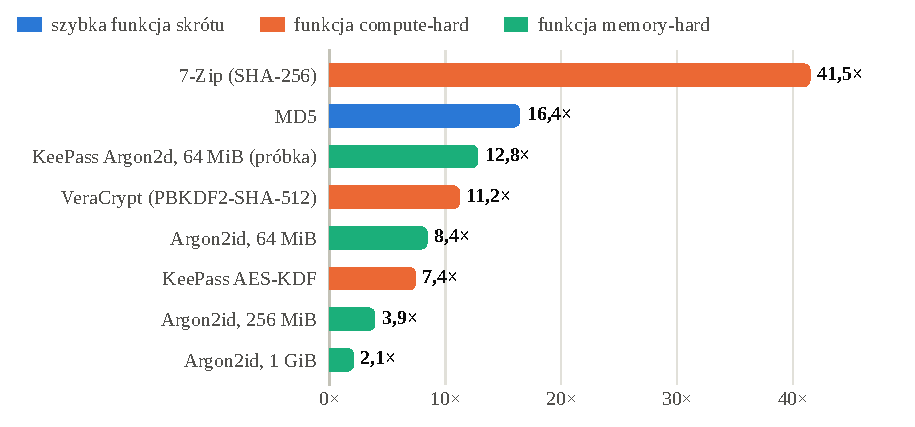
\includegraphics[width=\textwidth]{rysunki/r5-gpu-cpu.pdf}
\caption{Przewaga GPU nad CPU dla wszystkich badanych funkcji, uporządkowana malejąco}
\label{rys:gpu-cpu}
\end{figure}

Przewaga GPU nie zależy wprost od podziału na funkcje compute-hard i~memory-hard, lecz od tego, jak dana funkcja odwzorowuje się na sprzęt:
\begin{itemize}
  \item \textbf{7-Zip daje najwyższą przewagę (41,5$\times$)}, ponieważ opiera się na funkcji SHA-256 wykonującej działania 32-bitowe, w~których procesory graficzne są szczególnie wydajne.
  \item \textbf{KeePass AES-KDF daje najniższą przewagę (7,4$\times$)}, ponieważ procesor Ryzen~5~5600 ma sprzętowe wsparcie szyfrowania AES (zestaw instrukcji AES-NI) i~wykonuje rundy AES bardzo wydajnie, przez co dystans do karty maleje.
  \item \textbf{VeraCrypt (11,2$\times$)} korzysta z~PBKDF2-HMAC-SHA-512, czyli działań 64-bitowych, mniej korzystnych dla konsumenckiej karty, więc procesor relatywnie nadrabia.
  \item \textbf{Argon2 przy 64~MiB daje jeszcze 8,4--12,8$\times$} na korzyść GPU, ponieważ przy tej ilości pamięci karta mieści wiele równoległych sprawdzeń; dopiero większa pamięć ujawnia własność memory-hard (podrozdział~\ref{sec:gpu-memory}). Różnica między wartością 12,8$\times$ z~próbki wbudowanej a~8,4$\times$ z~własnego skrótu wynika z~innych parametrów czasu ($t = 2$ wobec $t = 3$); porównywalny jest trend, nie wartości bezwzględne.
\end{itemize}

Wynika z~tego, że sama klasyfikacja funkcji jako memory-hard nie gwarantuje najmniejszej przewagi GPU przy niskich parametrach pamięci. Najskuteczniej ogranicza tę przewagę albo funkcja oparta na działaniach sprzętowo przyspieszanych w~procesorze (AES-KDF), albo -- co pokazała seria~4 -- funkcja memory-hard z~odpowiednio dużą pamięcią. Z~punktu widzenia obrońcy najpewniejszą ochroną jest funkcja memory-hard z~parametrem pamięci przekraczającym możliwości taniego sprzętu masowo równoległego: przy 1~GiB przewaga karty spadła do około dwukrotności, a~bezwzględna prędkość ataku -- do pojedynczych sprawdzeń na sekundę. Jest to ilościowe potwierdzenie zaleceń doboru funkcji wyprowadzania klucza, przyjętych w~warstwie ochrony danych opisanej w~rozdziale~\ref{ch:obrona}.

% =====================================================================
%  Rozdział 6 - wersja robocza do przeredagowania
%  Dane: wyniki/R6 (alarmy IDS, zbiór 60 plików, kontenery rzeczywiste),
%        wyniki/R4/r4.pcap i wyniki/R4/4.1 (nagrania ruchu)
%  Wszystkie liczby zweryfikowane z plików wyników i nagrań pcap.
%  Wykresy: tools/wykresy-praca.py r6
% =====================================================================
\chapter{Projekt i~weryfikacja wielowarstwowego systemu obronnego}\label{ch:obrona}

W rozdziale przedstawiono dwie warstwy detekcji zaprojektowane na podstawie wyników z~rozdziałów~\ref{ch:ataki} i~\ref{ch:gpu} oraz wyniki ich weryfikacji. Warstwa sieciowa wykrywa w~ruchu ślady zdarzeń zbadanych w~rozdziale~\ref{ch:ataki}: podszycie w~protokole ARP oraz zestawienie sesji TLS z~przestarzałą wersją protokołu lub słabym zestawem szyfrów. Warstwa danych rozpoznaje pliki zaszyfrowane wśród danych opuszczających organizację, co odpowiada końcowemu etapowi ataku -- wyprowadzeniu danych (ang. \ang{exfiltration}). Zaszyfrowanie lub spakowanie danych przed ich wyprowadzeniem ukrywa treść przed systemami ochrony przed wyciekiem danych (ang. \ang{Data Loss Prevention}, DLP), które analizują zawartość przesyłanych plików. Budowę systemu przedstawia rysunek~\ref{rys:warstwy}.

\begin{figure}[htbp]
\centering
\begin{tikzpicture}[
  font=\footnotesize,
  node distance=6mm and 7mm,
  warstwa/.style={draw, rounded corners=3pt, line width=0.8pt, inner xsep=6pt, inner ysep=7pt},
  blok/.style={draw, rounded corners=2pt, align=center, minimum height=11mm, text width=40mm, fill=black!4},
  wej/.style={draw, align=center, minimum height=11mm, text width=30mm},
  wyj/.style={draw, align=center, minimum height=11mm, text width=26mm, fill=black!10},
  etap/.style={draw, rounded corners=2pt, align=center, minimum height=11mm, text width=19mm, fill=black!4},
  strz/.style={-{Stealth[length=2mm]}, line width=0.7pt}
]
% --- warstwa sieciowa ---
\node[wej] (ruch) {kopia ruchu segmentu \kod{labnet} lub nagranie \kod{pcap}};
\node[blok, above right=1mm and 9mm of ruch.east, anchor=south west] (arp) {inspektor \kod{arp\_spoof}\\(wzorzec powiązań\\IP--MAC)};
\node[blok, below right=1mm and 9mm of ruch.east, anchor=north west] (tls) {reguły własne\\(sid 1000010--1000013)};
\path (arp.east |- ruch.east) ++(13mm,0) node[wyj, anchor=west] (al1) {alarmy czujnika\\(\kod{alert\_fast})};
\draw[strz] (ruch.east) -- ++(4.5mm,0) |- (arp.west);
\draw[strz] (ruch.east) -- ++(4.5mm,0) |- (tls.west);
\draw[strz] (arp.east) -- ++(4.5mm,0) |- (al1.west);
\draw[strz] (tls.east) -- ++(4.5mm,0) |- (al1.west);
\node[warstwa, fit=(ruch)(arp)(tls)(al1)] (w1) {};
\node[anchor=south west, font=\footnotesize\bfseries] at (w1.north west) {Warstwa sieciowa -- czujnik Snort~3 (podrozdział~\ref{sec:ids})};
% --- warstwa danych ---
\node[wej, below=17mm of tls.south -| ruch, anchor=north] (plik) {plik (treść opuszczająca organizację)};
\node[etap, right=6mm of plik] (h) {entropia\\$H \geq 7{,}5$};
\node[etap, right=5mm of h] (c) {$\chi^2 \leq 293{,}25$};
\node[etap, right=5mm of c] (m) {brak\\nagłówka};
\node[wyj, right=5mm of m, text width=20mm] (dec) {,,dane zaszyfrowane''};
\draw[strz] (plik) -- (h); \draw[strz] (h) -- (c); \draw[strz] (c) -- (m); \draw[strz] (m) -- (dec);
\node[warstwa, fit=(plik)(h)(c)(m)(dec)] (w2) {};
\node[anchor=south west, font=\footnotesize\bfseries] at (w2.north west) {Warstwa danych -- klasyfikator entropijny B (podrozdział~\ref{sec:entropia})};
\end{tikzpicture}
\caption{Budowa dwuwarstwowego systemu detekcji}
\label{rys:warstwy}
\end{figure}

Obie warstwy weryfikowano offline: warstwę sieciową na nagraniach ruchu zarejestrowanych przez czujnik w~trakcie eksperymentów z~rozdziału~\ref{ch:ataki}, a~warstwę danych na zbiorze plików testowych oraz na rzeczywistych plikach zaszyfrowanych utworzonych w~rozdziale~\ref{ch:gpu}. Taki sposób weryfikacji pozwala wielokrotnie uruchamiać detekcję na identycznym materiale (podrozdział~\ref{sec:czujnik}).

% ---------------------------------------------------------------------
\section{Detekcja w~warstwie sieciowej}\label{sec:ids}

\subsection*{Konfiguracja czujnika}

Detekcję w~warstwie sieciowej realizuje Snort~3.12.2.0~\cite{snort3} na maszynie \kod{sensor} -- otwarty system IDS, którego właściwości porównano z~systemem Suricata m.in. w~pracy~\cite{boukebous2023}. Ustawienia laboratorium (plik \kod{lab.lua}) obejmują trzy elementy:
\begin{itemize}
  \item zmienną \kod{HOME\_NET} ustawioną na sieć laboratorium 10.10.10.0/24;
  \item inspektor \kod{arp\_spoof} ze wzorcem powiązań adresów IP i~MAC klienta oraz serwera (tabela~\ref{tab:arp-wzorzec});
  \item włączone reguły wbudowane, do których należą alarmy inspektora \kod{arp\_spoof} (identyfikator generatora 112), oraz dołączony plik reguł własnych \kod{local.rules}.
\end{itemize}

Reguły własne wykrywają w~komunikacie ServerHello, wysyłanym przez serwer w~odpowiedzi na ofertę klienta, wersję protokołu i~zestaw szyfrów wybrane przez serwer. Komunikat ten jest przesyłany jawnie we wszystkich wersjach protokołu, również w~TLS~1.3. Położenie pól wykorzystywanych przez reguły podano w~tabeli~\ref{tab:serverhello}.

\begin{table}[htbp]
\centering\small
\begin{tabularx}{\textwidth}{@{}l l L@{}}
\toprule
\textbf{Bajty} & \textbf{Pole} & \textbf{Wartość wykorzystywana w~regułach} \\
\midrule
0       & typ rekordu TLS & \kod{0x16} (rekord uzgadniania) \\
1--2    & wersja rekordu & \kod{0x03 0xXX} \\
3--4    & długość rekordu & -- \\
5       & typ komunikatu & \kod{0x02} (ServerHello) \\
6--8    & długość komunikatu & -- \\
9--10   & wersja protokołu wybrana przez serwer & \kod{0x0300} -- SSLv3, \kod{0x0301} -- TLS~1.0, \kod{0x0302} -- TLS~1.1 \\
11--42  & wartość losowa serwera (32~B) & -- \\
43      & długość identyfikatora sesji ($n$) & -- \\
44+$n$, 45+$n$ & wybrany zestaw szyfrów & \kod{0xC014} -- \kod{ECDHE-RSA-AES256-SHA} \\
\bottomrule
\end{tabularx}
\caption{Pola komunikatu ServerHello liczone od początku rekordu TLS}
\label{tab:serverhello}
\end{table}

Reguły wersji (sid 1000010--1000012) sprawdzają kolejno: typ rekordu, typ komunikatu i~wartość pola wersji. W~TLS~1.3 pole to zawiera zawsze wartość \kod{0x0303}, a~rzeczywista wersja jest przenoszona w~rozszerzeniu \ang{supported\_versions}. Wartości \kod{0x0303} nie można więc użyć do odróżnienia TLS~1.2 od TLS~1.3 i~reguły celowo pomijają ją, ograniczając się do wartości oznaczających wersje przestarzałe: SSLv3, TLS~1.0 i~TLS~1.1, z~których dwie ostatnie formalnie wycofał RFC~8996~\cite{rfc8996}. Reguła słabego szyfru (sid 1000013) szuka bajtów \kod{0xC014} w~oknie zaczynającym się 30~bajtów za polem typu komunikatu, czyli od 36. bajtu rekordu. Położenie zestawu szyfrów zależy od długości identyfikatora sesji; w~badanym nagraniu reguła dopasowała go zarówno na pozycji 44 (identyfikator pusty), jak i~76 (identyfikator 32-bajtowy). Okno obejmuje także końcówkę pola losowego i~identyfikator sesji, dlatego reguła jest heurystyką: przypadkowe wystąpienie tych bajtów w~polach losowych spowodowałoby fałszywy alarm. Treść reguł przedstawia listing~\ref{lst:reguly}; reguły 1000011 i~1000012 różnią się od 1000010 wyłącznie treścią komunikatu i~szukaną wartością wersji (\kod{|03 01|}, \kod{|03 02|}).

\begin{lstlisting}[float=htbp, caption={Reguły własne czujnika do wykrywania przestarzałych parametrów sesji TLS (fragment pliku \kod{local.rules})}, label={lst:reguly}]
alert tcp any any -> any any ( msg:"LAB 6.1 - ServerHello: wynegocjowano SSLv3 (przestarzaly protokol)";
    flow:to_client,established;
    content:"|16 03|", offset 0, depth 2;
    content:"|02|", offset 5, depth 1;
    content:"|03 00|", offset 9, depth 2;
    sid:1000010; rev:1; )

alert tcp any any -> any any ( msg:"LAB 6.1 - ServerHello: wynegocjowano slaby szyfr ECDHE-RSA-AES256-SHA (CBC/SHA1)";
    flow:to_client,established;
    content:"|16 03|", offset 0, depth 2;
    content:"|02|", offset 5, depth 1;
    content:"|c0 14|", distance 30, within 60;
    sid:1000013; rev:1; )
\end{lstlisting}

\subsection*{Materiał testowy}

Reguły i~inspektor uruchomiono offline na nagraniu \kod{r4.pcap}, zarejestrowanym przez czujnik 25.10.2026 w~czasie eksperymentów z~podrozdziałów~\ref{sec:tlsneg}--\ref{sec:lenext}. Nagranie trwa około 34~minut (2064~s) i~zawiera 10\,261 pakietów, w~tym:
\begin{itemize}
  \item 15 komunikatów ServerHello obu serwerów: po 7 z~dwóch przebiegów skanu wersji protokołu (podrozdział~\ref{sec:tlsneg}) i~jeden z~dodatkowego połączenia TLS~1.3 z~serwerem utwardzonym, zarejestrowanego między przebiegami;
  \item 827 żądań HTTP \kod{GET} do aplikacji testowej (10.10.10.30, port 5000) z~eksperymentów dotyczących integralności;
  \item 8 ramek ARP -- cztery pary zapytanie--odpowiedź wymieniane przez klienta i~serwer w~trakcie zwykłej pracy; wszystkie zawierają poprawne powiązania adresów, zgodne ze wzorcem.
\end{itemize}
Nagranie nie zawiera zatem żadnej próby podszycia w~ARP. Detekcję takiej próby zweryfikowano na osobnym nagraniu \kod{arp41.pcap} z~podrozdziału~\ref{sec:arp}.

\subsection*{Wyniki}

Na nagraniu \kod{r4.pcap} czujnik zgłosił 15~alarmów: 12 z~reguł własnych i~3 z~inspektora \kod{arp\_spoof}. Alarmy reguł własnych przedstawia rysunek~\ref{rys:snort-tls}, a~ich przyporządkowanie do poszczególnych komunikatów ServerHello -- tabela~\ref{tab:ids-serverhello}. Zestaw szyfrów każdego komunikatu odczytano bezpośrednio z~nagrania.

\begin{figure}[htbp]
\centering
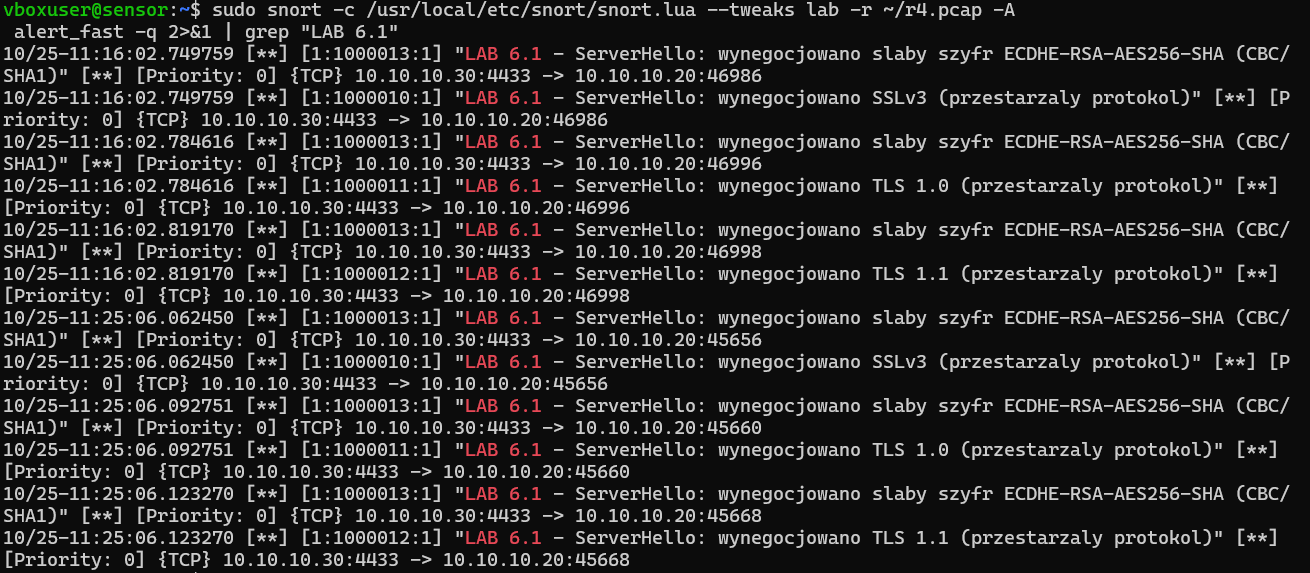
\includegraphics[width=\textwidth]{rysunki/r6-snort-tls.png}
\caption{Alarmy reguł własnych na nagraniu \kod{r4.pcap} (wyjście programu Snort przefiltrowane do reguł ,,LAB 6.1'')}
\label{rys:snort-tls}
\end{figure}

\begin{table}[htbp]
\centering\small
\begin{tabularx}{\textwidth}{@{}l l L c l@{}}
\toprule
\textbf{Serwer} & \textbf{Wersja} & \textbf{Zestaw szyfrów} & \textbf{Liczba} & \textbf{Alarmy (sid)} \\
\midrule
:443  & TLS~1.2 & \kod{ECDHE-RSA-AES128-GCM-SHA256} (\kod{0xC02F}) & 2 & brak \\
:443  & TLS~1.3 & \kod{TLS\_AES\_256\_GCM\_SHA384} (\kod{0x1302}) & 3 & brak \\
:4433 & SSLv3   & \kod{ECDHE-RSA-AES256-SHA} (\kod{0xC014}) & 2 & 1000010, 1000013 \\
:4433 & TLS~1.0 & \kod{ECDHE-RSA-AES256-SHA} (\kod{0xC014}) & 2 & 1000011, 1000013 \\
:4433 & TLS~1.1 & \kod{ECDHE-RSA-AES256-SHA} (\kod{0xC014}) & 2 & 1000012, 1000013 \\
:4433 & TLS~1.2 & \kod{ECDHE-RSA-AES256-GCM-SHA384} (\kod{0xC030}) & 4 & brak \\
\midrule
\multicolumn{3}{@{}l}{\textbf{Razem}} & \textbf{15} & \textbf{12 alarmów} \\
\bottomrule
\end{tabularx}
\caption{Komunikaty ServerHello w~nagraniu \kod{r4.pcap} i~wywołane przez nie alarmy}
\label{tab:ids-serverhello}
\end{table}

Każdy z~sześciu komunikatów z~przestarzałą wersją protokołu wywołał alarm reguły wersji (po dwa dla SSLv3, TLS~1.0 i~TLS~1.1) i~alarm reguły słabego szyfru, ponieważ we wszystkich tych sesjach serwer wybrał zestaw \kod{ECDHE-RSA-AES256-SHA}. Dziewięć pozostałych komunikatów -- wszystkie z~serwera utwardzonego oraz sesje TLS~1.2 serwera przestarzałego z~zestawem AEAD -- nie wywołało żadnego alarmu. Reguły własne wykryły więc 6 z~6 sesji z~przestarzałymi parametrami, nie zgłaszając żadnego fałszywego alarmu dla 9 sesji poprawnych. Heurystyczne okno reguły 1000013 nie spowodowało w~nagraniu przypadkowych dopasowań: bajty \kod{0xC014} wystąpiły w~danych komunikatów ServerHello wyłącznie w~polu zestawu szyfrów.

Trzy alarmy inspektora \kod{arp\_spoof} to alarmy o~identyfikatorze 112:1 (,,\ang{unicast ARP request}''). Ich znaczniki czasu odpowiadają dokładnie trzem zapytaniom ARP w~nagraniu, które zostały wysłane bezpośrednio na znany adres sprzętowy odbiorcy zamiast na adres rozgłoszeniowy (tabela~\ref{tab:ids-arp}). Zapytania takie wysyła system Linux przy sprawdzaniu aktualności wpisu w~tablicy sąsiadów, a~klient i~serwer pracują pod kontrolą systemu Ubuntu. Wszystkie trzy zawierały poprawne powiązania adresów, są to więc fałszywe alarmy.

\begin{table}[htbp]
\centering\small
\begin{tabularx}{\textwidth}{@{}r l l l L@{}}
\toprule
\textbf{Czas [s]} & \textbf{Operacja} & \textbf{Nadawca} & \textbf{Adresat ramki} & \textbf{Alarm} \\
\midrule
27,679  & zapytanie  & 10.10.10.20 & rozgłoszeniowy & brak \\
27,680  & odpowiedź  & 10.10.10.30 & 10.10.10.20 & brak \\
341,735 & zapytanie  & 10.10.10.20 & 10.10.10.30 (unicast) & 112:1 \\
341,736 & odpowiedź  & 10.10.10.30 & 10.10.10.20 & brak \\
341,926 & zapytanie  & 10.10.10.30 & 10.10.10.20 (unicast) & 112:1 \\
341,927 & odpowiedź  & 10.10.10.20 & 10.10.10.30 & brak \\
576,669 & zapytanie  & 10.10.10.30 & 10.10.10.20 (unicast) & 112:1 \\
576,670 & odpowiedź  & 10.10.10.20 & 10.10.10.30 & brak \\
\bottomrule
\end{tabularx}
\caption{Ramki ARP w~nagraniu \kod{r4.pcap} (czas od początku nagrania; wszystkie powiązania zgodne ze wzorcem)}
\label{tab:ids-arp}
\end{table}

Zestawienie skuteczności warstwy sieciowej na obu nagraniach zawiera tabela~\ref{tab:ids-bilans}. W~nagraniu \kod{r4.pcap} trafnych było 12 z~15~alarmów. Wszystkie alarmy fałszywe pochodziły z~alarmu 112:1, który zgłasza każde zapytanie typu unicast, niezależnie od tego, czy zawarte w~nim powiązanie jest poprawne. Alarmy 112:3 i~112:4, które wskazały próbę podszycia w~podrozdziale~\ref{sec:arp}, na zwykłym ruchu nie wystąpiły ani razu.

\begin{table}[htbp]
\centering\small
\begin{tabularx}{\textwidth}{@{}L l c c@{}}
\toprule
\textbf{Zdarzenie} & \textbf{Nagranie} & \textbf{Wykryte} & \textbf{Fałszywe alarmy} \\
\midrule
podszycie w~ARP (alarmy 112:3, 112:4) & \kod{arp41.pcap} & 3 z~3 ramek & 0 (3 ogłoszenia) \\
zwykły ruch ARP (alarm 112:1) & \kod{r4.pcap} & -- & 3 (z~8 ramek) \\
przestarzała wersja TLS (1000010--1000012) & \kod{r4.pcap} & 6 z~6 sesji & 0 (z~9 sesji) \\
słaby zestaw szyfrów (1000013) & \kod{r4.pcap} & 6 z~6 sesji & 0 (z~9 sesji) \\
\bottomrule
\end{tabularx}
\caption{Skuteczność warstwy sieciowej}
\label{tab:ids-bilans}
\end{table}

% ---------------------------------------------------------------------
\section{Detekcja prób eksfiltracji na podstawie analizy entropii}\label{sec:entropia}

\subsection*{Cechy i~klasyfikatory}

Warstwa danych ocenia, czy plik zawiera dane zaszyfrowane, na podstawie rozkładu wartości jego bajtów. Wykorzystywane są trzy cechy:
\begin{itemize}
  \item \textbf{entropia Shannona} $H = -\sum_{i=0}^{255} p_i \log_2 p_i$, gdzie $p_i$ to udział bajtów o~wartości~$i$; wynosi od 0 do 8~bitów na bajt, a~wartość bliską 8 mają dane o~rozkładzie zbliżonym do losowego~\cite{davies2022};
  \item \textbf{statystyka chi-kwadrat} $\chi^2 = \sum_{i=0}^{255} (n_i - E)^2 / E$, gdzie $n_i$ to liczba bajtów o~wartości~$i$, a~$E = N/256$ to liczba oczekiwana przy rozkładzie jednostajnym dla pliku o~długości $N$; mierzy odstępstwo rozkładu od jednostajnego;
  \item \textbf{rozpoznany nagłówek} -- obecność na początku pliku sygnatury znanego formatu (gzip, zip, 7z, PNG, JPEG, PDF, bzip2, xz, RAR).
\end{itemize}

Porównano dwa klasyfikatory, dla których klasą pozytywną są dane zaszyfrowane:
\begin{itemize}
  \item \textbf{klasyfikator A} -- plik jest zaszyfrowany, jeżeli $H \geq 7{,}5$;
  \item \textbf{klasyfikator B} -- plik jest zaszyfrowany, jeżeli $H \geq 7{,}5$, $\chi^2 \leq 293{,}25$ i~nie rozpoznano nagłówka.
\end{itemize}
Próg $\chi^2$ to kwantyl rzędu 0,95 rozkładu chi-kwadrat o~255 stopniach swobody (293,248). Dla danych o~rozkładzie jednostajnym statystyka $\chi^2$ przekracza ten próg z~prawdopodobieństwem około 5\%. Obliczenia wykonują skrypty \kod{r6-entropia.py} (zbiór testowy) i~\kod{r6-realne.py} (pliki rzeczywiste), napisane w~języku Python z~użyciem wyłącznie biblioteki standardowej.

\subsection*{Zbiór testowy}

Zbiór testowy wygenerował skrypt \kod{r6-gen-zbior.py}. Zawiera on 60 plików w~trzech grupach po 20 (tabela~\ref{tab:zbior}). Treść plików jawnych i~rozmiary plików zaszyfrowanych wyznacza generator pseudolosowy o~stałym ziarnie 20261029. Zawartość plików zaszyfrowanych pochodzi z~systemowego generatora liczb losowych (\kod{os.urandom}), który modeluje wynik działania dobrego szyfru; nie jest ona odtwarzalna bit po bicie.

\begin{table}[htbp]
\centering\small
\begin{tabularx}{\textwidth}{@{}l L r@{}}
\toprule
\textbf{Grupa} & \textbf{Zawartość} & \textbf{Rozmiar [B]} \\
\midrule
jawne (20) & tekst, kod w~języku Python, CSV, JSON, dziennik serwera, HTML -- po kolei & 6\,189--39\,287 \\
skompresowane (20) & pliki jawne po kompresji: gzip (10 plików) i~zip (10 plików), stopień kompresji 9 & 740--9\,084 \\
zaszyfrowane (20) & dane losowe bez nagłówka & 8\,573--62\,991 \\
\bottomrule
\end{tabularx}
\caption{Skład zbioru testowego}
\label{tab:zbior}
\end{table}

\subsection*{Wyniki}

Średnie wartości cech oraz ich zakresy w~grupach podano w~tabeli~\ref{tab:cechy}, a~położenie wszystkich plików w~przestrzeni cech -- na rysunku~\ref{rys:rozrzut}. Pliki skompresowane i~zaszyfrowane mają zbliżoną, wysoką entropię, a~ich zakresy niemal się stykają: najwyższa entropia pliku skompresowanego wynosi 7,9778, a~najniższa pliku zaszyfrowanego -- 7,9780~bitu na bajt. Rozdzielenie tych grup samą entropią wymagałoby więc progu dobranego z~dokładnością do 0,0002~bitu na bajt pod ten konkretny zbiór, co nie ma praktycznego znaczenia; trudność odróżnienia danych skompresowanych od zaszyfrowanych na podstawie entropii opisano również w~literaturze~\cite{degaspari2022}. Grupy różnią się natomiast statystyką $\chi^2$: wszystkie pliki zaszyfrowane leżą poniżej progu, a~większość plików skompresowanych -- powyżej.

\begin{table}[htbp]
\centering\small
\begin{tabular}{@{}lrrrr@{}}
\toprule
\textbf{Grupa} & \textbf{Średnia $H$} & \textbf{Zakres $H$} & \textbf{Średnia $\chi^2$} & \textbf{Zakres $\chi^2$} \\
\midrule
jawne         & 4,331 & 3,8582--4,6308 & 439\,854,8 & 124\,783,8--726\,731,3 \\
skompresowane & 7,815 & 7,2486--7,9778 & 575,0      & 251,3--1\,636,9 \\
zaszyfrowane  & 7,994 & 7,9780--7,9972 & 257,3      & 223,4--284,3 \\
\bottomrule
\end{tabular}
\caption{Entropia [bit/bajt] i~statystyka $\chi^2$ w~grupach zbioru testowego}
\label{tab:cechy}
\end{table}

\begin{figure}[htbp]
\centering
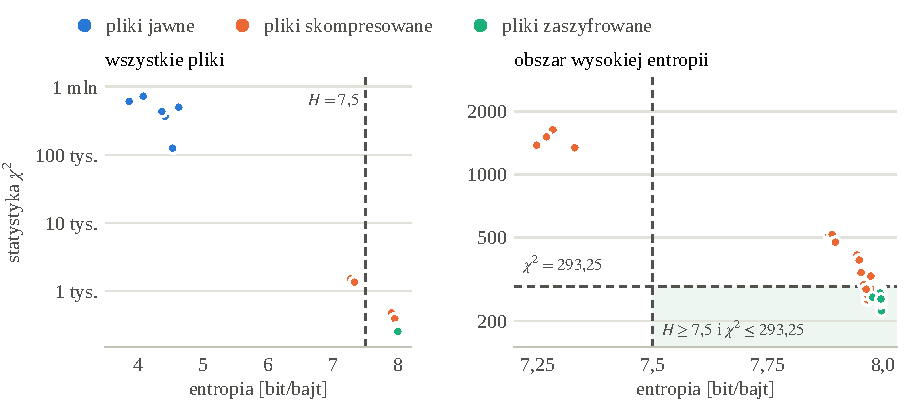
\includegraphics[width=\textwidth]{rysunki/r6-rozrzut.pdf}
\caption{Pliki zbioru testowego w~przestrzeni cech; prawy panel powiększa obszar wysokiej entropii, zacieniowano obszar spełniający oba progi klasyfikatora B}
\label{rys:rozrzut}
\end{figure}

Działanie kolejnych warunków klasyfikatora B przedstawia rysunek~\ref{rys:etapy}. Warunek entropii odrzucił wszystkie pliki jawne oraz cztery najmniejsze archiwa zip (740--751~B), przepuszczając 16 plików skompresowanych. Warunek $\chi^2$ odrzucił 11 z~nich. Pozostałe 5 plików to archiwa gzip, których statystyka $\chi^2$ nie przekroczyła progu (251,3--283,4); odrzuciło je dopiero rozpoznanie nagłówka. Wszystkie 20 plików zaszyfrowanych spełniło wszystkie trzy warunki.

\begin{figure}[htbp]
\centering
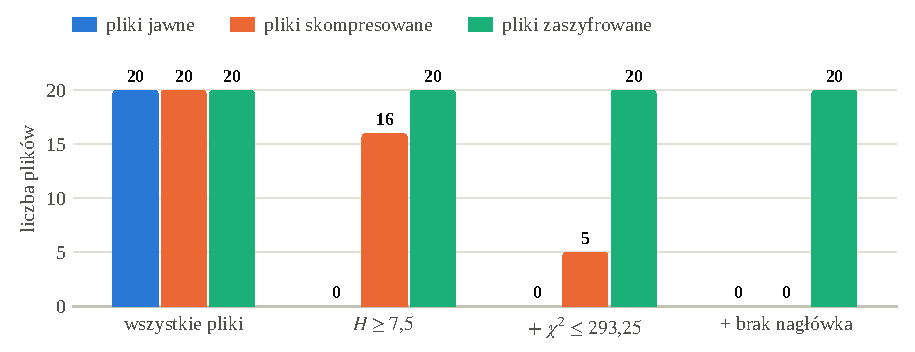
\includegraphics[width=\textwidth]{rysunki/r6-etapy.pdf}
\caption{Liczba plików uznanych za zaszyfrowane po kolejnych warunkach klasyfikatora B}
\label{rys:etapy}
\end{figure}

Macierze pomyłek i~miary jakości obu klasyfikatorów zawiera tabela~\ref{tab:klasyfikatory}, a~wynik działania skryptu -- rysunek~\ref{rys:entropia}. Klasyfikator A wykrył wszystkie pliki zaszyfrowane, ale uznał za zaszyfrowane także 16 z~20 plików skompresowanych, co daje 40\% fałszywych alarmów wśród 40 plików niezaszyfrowanych. Klasyfikator B rozpoznał wszystkie pliki poprawnie.

\begin{table}[htbp]
\centering\small
\begin{tabular}{@{}lcc@{}}
\toprule
\textbf{Miara} & \textbf{Klasyfikator A} & \textbf{Klasyfikator B} \\
\midrule
prawdziwie pozytywne (TP)  & 20 & 20 \\
fałszywie pozytywne (FP)   & 16 & 0 \\
prawdziwie negatywne (TN)  & 24 & 40 \\
fałszywie negatywne (FN)   & 0  & 0 \\
\midrule
czułość, TP/(TP+FN)                 & 100,0\% & 100,0\% \\
odsetek fałszywych alarmów, FP/(FP+TN) & 40,0\% & 0,0\% \\
precyzja, TP/(TP+FP)                & 55,6\%  & 100,0\% \\
dokładność, (TP+TN)/60              & 73,3\%  & 100,0\% \\
\bottomrule
\end{tabular}
\caption{Macierze pomyłek i~miary jakości klasyfikatorów na zbiorze testowym}
\label{tab:klasyfikatory}
\end{table}

\begin{figure}[htbp]
\centering
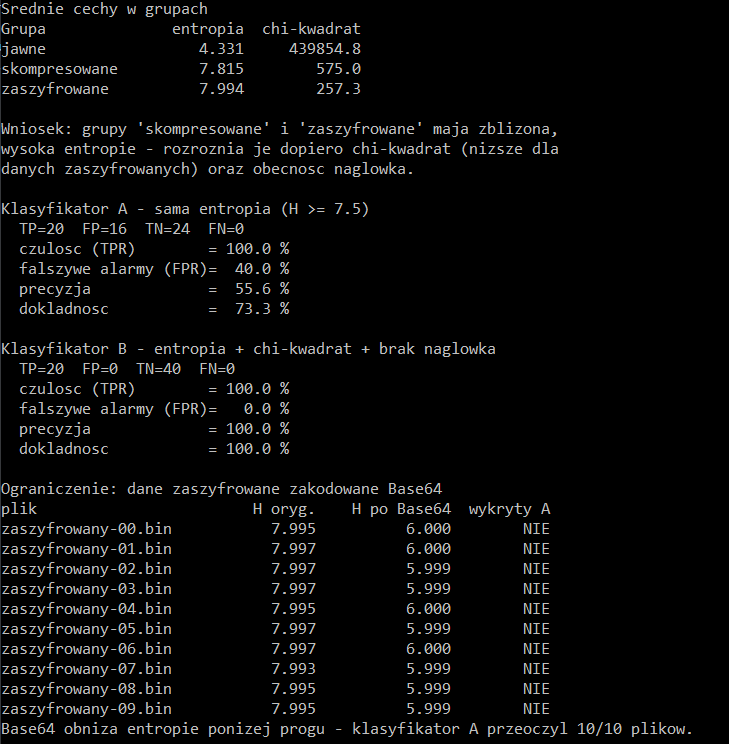
\includegraphics[width=0.72\textwidth]{rysunki/r6-entropia.png}
\caption{Wynik działania skryptu \kod{r6-entropia.py} na zbiorze testowym}
\label{rys:entropia}
\end{figure}

Skrypt sprawdzał również wpływ kodowania Base64, stosowanego do przesyłania danych binarnych w~kanałach tekstowych (np. w~poczcie elektronicznej lub w~treści żądań HTTP). Dziesięć pierwszych plików zaszyfrowanych zakodowano w~Base64 i~ponownie wyznaczono entropię. We wszystkich przypadkach spadła ona z~7,993--7,997 do 5,999--6,000~bitów na bajt, ponieważ alfabet Base64 liczy 64~znaki, a~$\log_2 64 = 6$. Wszystkie 10 plików znalazło się poniżej progu entropii i~nie zostało wykrytych. Dotyczy to obu klasyfikatorów, ponieważ warunek entropii jest częścią każdego z~nich.

\subsection*{Pliki rzeczywiste}

Zbiór testowy modeluje dane zaszyfrowane jako dane losowe bez nagłówka. Aby sprawdzić klasyfikatory na rzeczywistych plikach zaszyfrowanych, uruchomiono je na dziewięciu plikach utworzonych w~rozdziale~\ref{ch:gpu}: trzech kontenerach VeraCrypt, pięciu bazach KeePass i~archiwum 7-Zip z~hasłem. Do listy rozpoznawanych nagłówków dodano sygnaturę formatu KDBX. Pliki analizowano w~całości, ponieważ żaden nie przekraczał przyjętej wielkości próbki (8~MiB). Wyniki zawiera tabela~\ref{tab:realne}.

\begin{table}[htbp]
\centering\small
\begin{tabular}{@{}lrrrlcc@{}}
\toprule
\textbf{Plik} & \textbf{Rozmiar [B]} & \textbf{$H$} & \textbf{$\chi^2$} & \textbf{Nagłówek} & \textbf{A} & \textbf{B} \\
\midrule
\kod{kp-aeskdf-kdbx31.kdbx} & 1\,390 & 7,8442 & 342,7  & KDBX & tak & nie \\
\kod{kp-aeskdf-kdbx4.kdbx}  & 1\,656 & 7,7857 & 956,9  & KDBX & tak & nie \\
\kod{kp-argon2d-64.kdbx}    & 1\,990 & 7,7553 & 1\,602,7 & KDBX & tak & nie \\
\kod{kp-argon2d-256.kdbx}   & 1\,526 & 7,6398 & 2\,059,0 & KDBX & tak & nie \\
\kod{kp-argon2d-1024.kdbx}  & 1\,846 & 7,7346 & 1\,706,1 & KDBX & tak & nie \\
\kod{test-7zip.7z}          & 5\,263 & 7,9544 & 337,2  & 7z   & tak & nie \\
\kod{vc-sha512-pim1.hc}     & 2\,097\,152 & 7,9999 & 267,1 & -- & tak & tak \\
\kod{vc-sha512-pim250.hc}   & 2\,097\,152 & 7,9999 & 248,7 & -- & tak & tak \\
\kod{vc-sha512-pim500.hc}   & 2\,097\,152 & 7,9999 & 283,0 & -- & tak & tak \\
\bottomrule
\end{tabular}
\caption{Klasyfikatory A i~B na rzeczywistych plikach zaszyfrowanych}
\label{tab:realne}
\end{table}

Klasyfikator A uznał za zaszyfrowane wszystkie 9 plików, a~klasyfikator B -- tylko 3 kontenery VeraCrypt. Kontenery te nie mają nagłówka rozpoznawalnego po sygnaturze, a~ich rozkład bajtów odpowiada danym losowym. Bazy KeePass i~archiwum 7-Zip zaczynają się sygnaturą swojego formatu, więc klasyfikator B odrzucił je już na podstawie nagłówka; ponadto wszystkie miały statystykę $\chi^2$ powyżej progu. Wynik pokazuje, że warunek braku nagłówka, który na zbiorze testowym eliminował fałszywe alarmy dla archiwów, powoduje jednocześnie pominięcie zaszyfrowanych formatów mających własny nagłówek. Formaty takie wymagają osobnej reguły systemu DLP, uwzględniającej budowę formatu: baza KeePass jest zawsze zaszyfrowana, więc wystarcza sama sygnatura, natomiast archiwum 7-Zip może, ale nie musi być zaszyfrowane.

% ---------------------------------------------------------------------
\section{Weryfikacja skuteczności systemu}\label{sec:weryfikacja}

Tabela~\ref{tab:pokrycie} zestawia zagrożenia zbadane w~rozdziałach~\ref{ch:ataki} i~\ref{ch:gpu} z~mechanizmami, które je ograniczają. Część zagrożeń jest wykrywana przez warstwy detekcji opisane w~tym rozdziale, a~części zapobiegają poprawione konfiguracje i~mechanizmy kryptograficzne zbadane wcześniej.

\begin{table}[htbp]
\centering\small
\begin{tabularx}{\textwidth}{@{}>{\raggedright\arraybackslash}p{3.3cm} >{\raggedright\arraybackslash}p{3.6cm} L@{}}
\toprule
\textbf{Zagrożenie} & \textbf{Mechanizm} & \textbf{Wynik weryfikacji} \\
\midrule
podszycie w~ARP & detekcja: inspektor \kod{arp\_spoof} & 3 z~3 ramek wykryte; 3 fałszywe alarmy 112:1 na zwykłym ruchu \\
sesja z~przestarzałą wersją TLS & detekcja: reguły 1000010--1000012 & 6 z~6 sesji wykryte, 0 fałszywych alarmów na 9 sesjach poprawnych \\
& zapobieganie: wyłączenie wersji starszych niż TLS~1.2 & serwer utwardzony przyjmuje tylko TLS~1.2 i~1.3 (podrozdział~\ref{sec:tlsneg}) \\
słaby zestaw szyfrów & detekcja: reguła 1000013 & 6 z~6 sesji wykryte, 0 fałszywych alarmów \\
modyfikacja ciasteczka & zapobieganie: tryb AES-GCM & 0 z~400 modyfikacji przyjętych (podrozdziały~\ref{sec:ctr}, \ref{sec:cbc}); brak detekcji w~warstwie sieciowej \\
podpis żądania API & zapobieganie: HMAC-SHA-256 & konstrukcja odporna na atak przedłużenia (podrozdział~\ref{sec:lenext}) \\
łamanie hasła offline & zapobieganie: funkcja memory-hard z~dużą pamięcią & przewaga GPU nad CPU spada do 2,1$\times$ przy 1~GiB (podrozdział~\ref{sec:gpu-memory}) \\
eksfiltracja danych zaszyfrowanych & detekcja: klasyfikator B & zbiór testowy: 20 z~20 wykryte, 0 z~40 fałszywych alarmów; pliki rzeczywiste: 3 z~9 wykryte \\
\bottomrule
\end{tabularx}
\caption{Zagrożenia zbadane w~pracy i~mechanizmy, które je ograniczają}
\label{tab:pokrycie}
\end{table}

Warstwa sieciowa wykryła wszystkie badane zdarzenia: próbę podszycia w~ARP oraz wszystkie sesje z~przestarzałą wersją protokołu i~słabym zestawem szyfrów. Nie zgłosiła żadnego alarmu dla sesji serwera utwardzonego. Jej słabym punktem są alarmy 112:1, które stanowiły wszystkie 3 fałszywe alarmy w~nagraniu \kod{r4.pcap}. Warstwa danych w~wariancie B rozdzieliła bezbłędnie dane zaszyfrowane i~skompresowane w~zbiorze testowym, podczas gdy klasyfikator oparty na samej entropii dawał 40\% fałszywych alarmów. Na plikach rzeczywistych wykrył jednak tylko kontenery bez nagłówka.

Warstwy obejmują różne etapy ataku. Warstwa sieciowa wykrywa przygotowanie i~przeprowadzenie ataku w~sieci, czyli uzyskanie pozycji pośrednika i~zestawienie słabej sesji. Warstwa danych wykrywa próbę wyprowadzenia danych. Żadna z~nich nie wykrywa ataków na integralność danych aplikacji (podrozdziały~\ref{sec:ctr}--\ref{sec:lenext}) ani łamania haseł offline, które odbywa się poza siecią organizacji. Przed tymi zagrożeniami chronią wyłącznie mechanizmy zapobiegawcze: uwierzytelnione szyfrowanie, kod HMAC i~funkcje memory-hard. Uzasadnia to podejście wielowarstwowe, w~którym detekcja uzupełnia poprawną konfigurację kryptograficzną, a~nie ją zastępuje.

% ---------------------------------------------------------------------
\section{Ograniczenia rozwiązania}\label{sec:ograniczenia}

Weryfikacja ujawniła następujące ograniczenia, wynikające z~uzyskanych wyników lub z~budowy mechanizmów:
\begin{enumerate}
  \item \textbf{Kodowanie Base64 ukrywa dane zaszyfrowane.} Obniża ono entropię do około 6~bitów na bajt, przez co oba klasyfikatory przeoczyły 10 z~10 zakodowanych plików. Przed analizą entropii należałoby zdekodować typowe kodowania transportowe.
  \item \textbf{Formaty zaszyfrowane z~nagłówkiem nie są wykrywane przez klasyfikator B.} Bazy KeePass i~archiwum 7-Zip zostały odrzucone na podstawie nagłówka. Takie formaty wymagają osobnej reguły opartej na sygnaturze.
  \item \textbf{O~odróżnieniu części archiwów decyduje wyłącznie nagłówek.} Pięć archiwów gzip spełniło warunki entropii i~$\chi^2$. Dane skompresowane pozbawione nagłówka zostałyby więc uznane za zaszyfrowane.
  \item \textbf{Próg $\chi^2$ dopuszcza pominięcia.} Przy progu równym kwantylowi 0,95 około 5\% plików o~rozkładzie jednostajnym przekracza próg i~zostaje pominiętych. W~badanym zbiorze żaden z~20 plików zaszyfrowanych nie przekroczył progu, ale przy większej liczbie plików pominięcia są oczekiwane. Dla bardzo małych plików liczba bajtów przypadająca na jedną z~256 wartości jest mała, przez co rozkład statystyki słabiej zgadza się z~rozkładem chi-kwadrat.
  \item \textbf{Alarm 112:1 generuje fałszywe alarmy na zwykłym ruchu.} Zgłasza on każde zapytanie ARP typu unicast, w~tym zapytania wysyłane przy odświeżaniu tablicy sąsiadów. Alarm 112:4 działa tylko dla adresów wpisanych do wzorca, a~alarmy w~formacie \kod{alert\_fast} nie zawierają adresów, więc ich analiza wymaga sięgnięcia do nagrania.
  \item \textbf{Reguły TLS zależą od położenia pól w~pakiecie.} Zakładają, że rekord ServerHello zaczyna się na początku analizowanych danych (opcja \kod{offset 0}); w~nagraniu warunek ten był spełniony dla wszystkich 15 komunikatów. Reguła 1000013 jest ponadto heurystyką, która może dać fałszywy alarm przy przypadkowym wystąpieniu bajtów \kod{0xC014} w~polach losowych.
  \item \textbf{Reguła kontrolna ruchu HTTP nie zadziałała.} Plik reguł zawiera regułę kontrolną (sid 1000001) wykrywającą żądania \kod{GET} do aplikacji testowej. Mimo 827 takich żądań w~nagraniu nie wygenerowała ona żadnego alarmu. Przyczyny nie ustalono; reguła nie należy do ocenianej detekcji.
  \item \textbf{Zakres weryfikacji.} Obie warstwy weryfikowano offline, na nagraniach z~jednego stanowiska laboratoryjnego i~na syntetycznym zbiorze 60 plików uzupełnionym 9 plikami rzeczywistymi. Wyniki nie obejmują pracy czujnika na ruchu na żywo ani skuteczności na dużych, zróżnicowanych zbiorach danych.
\end{enumerate}

% Rozdział 7 - do napisania razem z rozdziałami 1-2
\chapter{Podsumowanie i wnioski}\label{ch:podsumowanie}
\section{Odpowiedzi na pytania badawcze}
\section{Rekomendacje dotyczące utwardzania systemów}
\section{Kierunki dalszych prac}


% ---------------- Literatura (bez numeru, w spisie treści) ----------------
\cleardoublepage
\phantomsection
\addcontentsline{toc}{chapter}{Literatura}
\bibliographystyle{unsrt}
\bibliography{bibliografia}

\end{document}
